\documentclass[final,5p,times,twocolumn]{elsarticle}

\usepackage[T1]{fontenc}
\usepackage[utf8]{inputenc}
\usepackage{amsmath,amssymb,amsfonts,amsthm}
\usepackage{mathtools}
\usepackage{graphicx}
\usepackage{booktabs}
\usepackage{multirow}
\usepackage{array}
\usepackage{xcolor}
\usepackage{microtype}
\usepackage{url}
\def\UrlBreaks{\do\/\do-\do\_\do.}
\usepackage[hidelinks]{hyperref}

\graphicspath{{figures/}}

\newtheorem{proposition}{Proposition}
\newtheorem{theorem}{Theorem}
\newtheorem{lemma}{Lemma}
\newtheorem{corollary}{Corollary}[theorem]
\theoremstyle{definition}
\newtheorem{definition}{Definition}
\theoremstyle{remark}
\newtheorem{remark}{Remark}
\newcounter{alg}

\newcommand{\SplitSlab}{\textup{\textsc{SplitSlab}}}
\newcommand{\RecallBench}{\textup{\textsc{RecallRegret-Bench}}}
\newcommand{\RMSNorm}{\operatorname{RMSNorm}}
\newcommand{\RoPE}{\operatorname{RoPE}}
\newcommand{\softmax}{\operatorname{softmax}}
\newcommand{\WAF}{\operatorname{WAF}}
\newcommand{\R}{\mathbb{R}}
\newcommand{\E}{\mathbb{E}}
\newcommand{\Prob}{\mathbb{P}}

\pdfstringdefDisableCommands{%
  \def\SplitSlab{SplitSlab}%
  \def\RecallBench{RecallRegret-Bench}%
}

\hyphenation{op-tical net-works semi-conduc-tor Paged-Attention Flash-Attention Dis-aggre-gated}
\setlength{\textfloatsep}{7pt plus 1pt minus 2pt}
\setlength{\dbltextfloatsep}{8pt plus 1pt minus 2pt}
\setlength{\floatsep}{6pt plus 1pt minus 2pt}

\journal{Future Generation Computer Systems}

\begin{document}

\begin{frontmatter}

\title{SplitSlab: Write-Once Canonical-Hash Residual Tiering to Eliminate Write Amplification and Compaction Regret in Disaggregated KV Stores}

\author[1]{Mohammed Kamran Syed\corref{cor1}}
\ead{mohammedkamran.syed@ieee.org}

\author[2]{Anudeep Rentala}
\ead{anudeep.rentala@ieee.org}

\author[2]{Somesh Rahul}
\ead{someshrahul@ieee.org}

\author[3]{Raghuram Malpe Pai}
\ead{raghuram.pai@ieee.org}

\author[3]{Krishna Suman Dara}
\ead{krishna-suman.dara@ieee.org}

\cortext[cor1]{Corresponding author (ORCID: 0009-0009-9058-5375).}

\affiliation[1]{organization={Independent Researcher},
                city={Mountain House},
                state={CA},
                postcode={95391},
                country={USA}}

\affiliation[2]{organization={Independent Researcher},
                city={Fremont},
                state={CA},
                postcode={94538},
                country={USA}}

\affiliation[3]{organization={Independent Researcher},
                city={Sunnyvale},
                state={CA},
                postcode={94086},
                country={USA}}

\begin{abstract}
Long-horizon Large Language Model (LLM) agent serving stacks pair online Key-Value (KV) eviction in GPU High-Bandwidth Memory (HBM) with content-addressed NVMe Solid-State Drive (SSD) offloading. Combining query-driven eviction with block-level flash storage violates three system invariants. Divergent agent queries prune different token subsets from shared prefixes and collapse fleet SHA-256 block deduplication to zero percent. Per-turn re-compaction dirties flash pages and induces 7.5x to 53.7x NVMe write amplification. Irreversible deletion of low-saliency early tokens causes compaction regret when later turns reference unqueried constants. We present SplitSlab, a canonical two-plane KV tiering engine that splits each immutable prefix block once into a 20 percent hot HBM anchor skeleton and a 64-kilobyte cold NVMe residual stripe, retaining a 64-byte bias-centered subspace sketch in HBM. During decoding, a parameter-free two-layer basis-aligned speculative query scores upcoming cold sketches and recalls needed stripes within the compute window whenever predictive entropy and prominence exceed threshold. On a unified-memory workstation prototype with uncached direct NVMe I/O across four 3B to 14B Qwen2.5 and Granite models, SplitSlab maintains 1.00x write amplification, 100 percent cross-agent deduplication, 77.4 to 79.6 percent steady HBM savings, and up to 95.0 percent delayed-recall recovery while recalling under 7 percent of cold stripes.
\end{abstract}

\begin{keyword}
Disaggregated KV-cache serving \sep NVMe write amplification \sep Content-addressed deduplication \sep KV-cache tiering \sep Subspace routing sketches \sep Large language model agents \sep Distributed storage systems
\end{keyword}

\end{frontmatter}

% ============================================================================
\section{Introduction}
% ============================================================================

Production serving engines for multi-turn coding, incident triage, and repository analysis agents~\cite{jimenez2024swebench,zheng2024sglang} process trajectories spanning tens of thousands of tokens. Because attention Key-Value (KV) state scales linearly with sequence length and batch size, operators pair two memory hierarchy optimizations: (i)~online KV compaction (\texttt{H2O}~\cite{zhang2023h2o}, \texttt{StreamingLLM}~\cite{xiao2024streamingllm}, \texttt{SnapKV}~\cite{li2024snapkv}), which retains roughly $20\%$ of high-attention tokens in GPU High-Bandwidth Memory (HBM) and discards the remaining $80\%$; and (ii)~disaggregated L2 KV offloading (\texttt{vLLM}~\cite{kwon2023vllm}, \texttt{DistServe}~\cite{zhong2024distserve}, \texttt{CacheGen}~\cite{liu2024cachegen}, \texttt{Mooncake}~\cite{qin2025mooncake}, \texttt{LMCache}~\cite{cheng2025lmcache}), which streams multi-megabyte KV slabs to NVMe Solid-State Drives (SSDs) indexed by the SHA-256 digest of the uncompacted token prefix~\cite{quinlan2002venti}.

Combining query-driven KV eviction with content-addressed NVMe offloading introduces three structural failures across the GPU-flash boundary:

\begin{enumerate}
  \item \emph{Prefix-Hash Collapse ($0\%$ Fleet Sharing):} Suppose Collaborating Agents~A and~B ingest the same shared repository snapshot in Turn~1, after which Agent~A inspects an ingress router module in Turn~2 while Agent~B inspects an OpenTelemetry exporter module. Online observation-window policies (\texttt{SnapKV}, \texttt{H2O}) rank Turn~1 keys using each agent's Turn~2 queries. Surviving token indices diverge immediately inside the first block, shifting every subsequent sequential slab boundary and reducing cross-agent SHA-256 slab deduplication from $100\%$ to $0.0\%$. In our $32$-agent fleet benchmark on \texttt{Qwen2.5-7B}, query-driven compaction writes $287.00$\,MB to flash, exceeding uncompacted \texttt{Full-KV} ($64.75$\,MB) by $4.43\times$.
  \item \emph{Flash Write Amplification ($7.5\times$--$53.7\times$ $\WAF$):} Block-interface NVMe SSDs and Zoned Namespaces (\texttt{ZNS})~\cite{hu2009waf,bjorling2021zns,rosenblum1992lfs} achieve peak bandwidth and endurance when writing immutable, page-aligned ($64$\,KB) sequential stripes once. Re-compacting KV state across $K$ conversational turns excises shifting token subsets from older slabs, forcing repeated $64$\,KB read-modify-write cycles ($7.54\times$--$20.13\times$ $\WAF$ across $12$--$24$ turns, rising to $53.67\times$ under ragged $24$\,KB per-head chunks).
  \item \emph{Compaction Regret on Delayed Recall:} Early background details such as an unused error trap (\texttt{LEGACY\_RENEG\_ABORT\_HEX = 0x7F3A}) receive low attention during intermediate coding turns (Turns~3--11) and are permanently deleted. When a canary crash dump surfaces \texttt{0x7F3A} at Turn~12, irreversible eviction baselines score $0.0\%$ exact match across all $72$ multi-model runs in our benchmark.
\end{enumerate}

\begin{figure*}[!t]
  \centering
  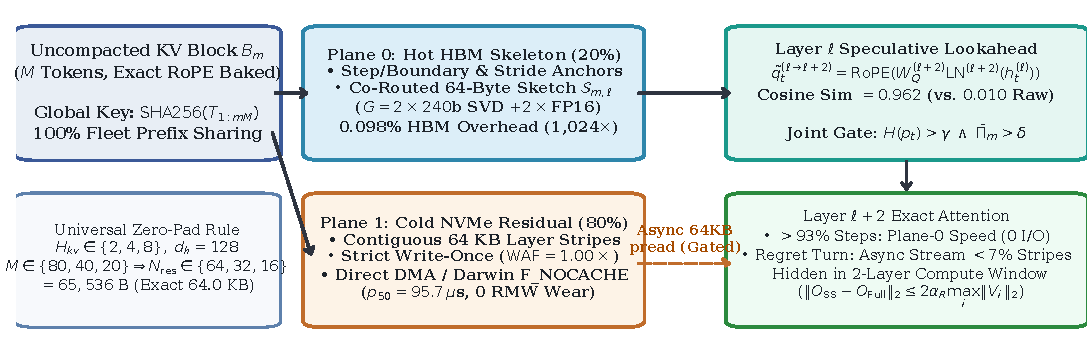
\includegraphics[width=0.92\textwidth]{fig1_architecture_overview.pdf}
  \caption{\SplitSlab{} canonical two-plane storage architecture and asynchronous recall pipeline. Completed prefix blocks $B_m$ ($M \in \{80,40,20\}$ tokens for Grouped-Query Attention with $H_{\mathrm{kv}} \in \{2,4,8\}$) split deterministically from prefix tokens alone into a $20\%$ Plane-0 HBM skeleton plus an exact $65{,}536$-byte ($64.0$\,KB) write-once Plane-1 NVMe stripe ($\WAF = 1.00\times$, $100\%$ SHA-256 fleet sharing). Each cold stripe retains a $64$-byte bias-centered subspace routing sketch $\mathcal{S}_{m,\ell}$ in HBM. At Layer~$\ell$, a parameter-free basis-aligned speculative query $\tilde{q}_t^{(\ell \to \ell+2)}$ scores Layer~$\ell+2$ sketches and streams needed $64$\,KB stripes within the two-layer compute window whenever predictive uncertainty $H(p_t) > \gamma$ and block prominence $\bar{\Pi}_m > \delta$.}
  \label{fig:arch_overview}
\end{figure*}

Existing recallable or sparse KV systems leave these storage constraints unresolved. \texttt{Quest}~\cite{tang2024quest} retains $100\%$ of KV pages in GPU HBM ($0\%$ HBM memory reduction) to skip attention compute~\cite{dao2022flashattention}. Node-local CPU DRAM offloaders including \texttt{FlexGen}~\cite{sheng2023flexgen}, \texttt{InfiniGen}~\cite{lee2024infinigen}, \texttt{ArkVale}~\cite{chen2024arkvale}, \texttt{ShadowKV}~\cite{sun2025shadowkv}, and \texttt{RetrievalAttention}~\cite{liu2024retrievalattention} rely on host DRAM capacity, construct per-head or query-dependent page layouts that prevent fleet-wide SHA-256 prefix sharing, or evaluate page digests synchronously at Layer~$\ell$ without hiding $100\,\mu\mathrm{s}$-class NVMe read latencies.

We present \SplitSlab{}, a write-once canonical-hash split-plane KV storage and speculative recall engine designed jointly for GPU HBM compaction and flash-friendly disaggregated NVMe pools. Fig.~\ref{fig:arch_overview} illustrates the design. \SplitSlab{} preserves global uncompacted prefix addressing while decoupling active HBM residency from irreversible deletion through four contributions:

\begin{enumerate}
  \item \emph{Zero-Padding Canonical Split-Plane Layout ($\WAF = 1.00\times$):} We formulate a universal Grouped-Query Attention (GQA)~\cite{ainslie2023gqa} stripe sizing rule that maps every standard KV head count $H_{\mathrm{kv}} \in \{2, 4, 8\}$ at head dimension $d_h = 128$ (FP16) to a logical block size $M \in \{80, 40, 20\}$ whose $80\%$ residual slice equals $65{,}536$ bytes ($64.0$\,KB) per layer with zero internal padding. Because Plane-0/Plane-1 partitioning uses only prefix-causal structural and stride rules, collaborating agents produce byte-identical Plane-0 skeletons and Plane-1 stripes ($100.0\%$ SHA-256 deduplication and $\WAF = 1.00\times$).
  \item \emph{Strict $64$-Byte Bias-Centered Sub-Cluster Sketch ($1{,}024\times$ Compression):} Each $64$\,KB cold stripe leaves a $64$-byte binary sketch $\mathcal{S}_{m,\ell}$ ($0.098\%$ HBM overhead) storing $G=2$ salience-weighted sub-cluster sign projections~\cite{charikar2002simhash,gao2024rabitq} across $240$ static $W_Q/W_K$ principal directions plus two FP16 norms. Deterministic cancellation of Rotary Position Embedding ($\RoPE$)~\cite{su2024roformer} key-projection bias ($\|b_K\|_2$ up to $920.5$ in \texttt{Qwen2.5}~\cite{yang2024qwen25}) and co-routing with resident Plane-0 anchors eliminate boundary blind spots.
  \item \emph{Parameter-Free Basis-Aligned Two-Layer Speculative Lookahead:} Directly scoring Layer~$\ell$ queries $q_t^{(\ell)}$ against Layer~$\ell+2$ key sketches yields $0.0102$ cosine similarity and $0.0\%$ recall accuracy due to independent per-layer head rotations. Projecting the Layer~$\ell$ residual stream through Layer~$\ell+2$'s static $\RMSNorm$ and $W_Q^{(\ell+2)}$ achieves $0.9623$ cosine similarity with zero trained parameters, hiding $72.7$--$189.1\,\mu\mathrm{s}$ uncached NVMe reads inside $2.03$--$5.17$\,ms two-layer compute windows.
  \item \emph{Formal Error, $\WAF$, and Multi-Model Hardware Verification:} We prove an exact Taylor-free attention perturbation bound $\|O_{\SplitSlab} - O_{\mathrm{FullKV}}\|_2 \le 2\alpha_R \max_i\|V_i\|_2$ (verified with zero violations across $560$ real attention heads), a greedy logit-margin equivalence condition, and linear $\Omega(K)$ re-compaction write amplification bounds. Across \texttt{Qwen2.5-3B}, \texttt{Qwen2.5-7B}, \texttt{Granite-3.1-8B}~\cite{mishra2024granite}, and \texttt{Qwen2.5-Coder-14B} using Darwin \texttt{F\_NOCACHE} uncached NVMe I/O, \SplitSlab{} saves $77.4\%$--$79.6\%$ of steady GPU HBM while recovering $45.0\%$--$95.0\%$ exact delayed recall ($55.0\%$--$95.0\%$ field accuracy) versus $0.0\%$ exact match for online eviction.
\end{enumerate}

The remainder of this paper covers related work in Section~\ref{sec:related}, the \SplitSlab{} architecture in Section~\ref{sec:arch} (Sections~\ref{subsec:layout}, \ref{subsec:sketch}, and~\ref{subsec:lookahead}), formal bounds in Section~\ref{sec:theory}, methodology in Section~\ref{sec:methodology}, evaluation in Section~\ref{sec:eval} (Sections~\ref{subsec:multimodel}, \ref{subsec:storage_eval}, \ref{subsec:ablations}, \ref{subsec:fleet_horizon}, and~\ref{subsec:revision_eval}), limitations in Section~\ref{sec:discussion}, and conclusions in Section~\ref{sec:conclusion}.

% ============================================================================
\section{Background and Related Work}\label{sec:related}
% ============================================================================

\begin{table*}[!t]
\centering
\caption{Architectural Comparison of KV-Cache Eviction, Sparse Attention, CPU Offloading, and Disaggregated NVMe Systems}
\label{tab:prior_art}
\footnotesize
\renewcommand{\arraystretch}{1.12}
\setlength{\tabcolsep}{4.0pt}
\resizebox{\textwidth}{!}{%
\begin{tabular}{@{}lcccccc@{}}
\toprule
\textbf{System / Paradigm} & \textbf{GPU HBM} & \textbf{Delayed-Recall} & \textbf{Offload Tier \&} & \textbf{Flash} & \textbf{Cross-Agent} & \textbf{Zero-Param Async} \\
 & \textbf{Savings} & \textbf{Recovery} & \textbf{Page Alignment} & $\mathbf{\WAF}$ & \textbf{SHA-256 Dedup} & \textbf{NVMe Lookahead} \\
\midrule
\texttt{vLLM}~\cite{kwon2023vllm}, \texttt{Mooncake}~\cite{qin2025mooncake}, \texttt{LMCache}~\cite{cheng2025lmcache} & $0\%$ & Yes ($100\%$) & NVMe / RDMA ($64$\,KB+) & $1.00\times$ & Yes ($100\%$) & N/A (Full HBM) \\
\texttt{H2O}~\cite{zhang2023h2o}, \texttt{StreamingLLM}~\cite{xiao2024streamingllm}, \texttt{SnapKV}~\cite{li2024snapkv} & $75\%$--$80\%$ & No ($0\%$) & None (Irreversible Drop) & N/A & No ($0\%$) & No \\
Online Evict + Naive NVMe Re-Compaction & $75\%$--$80\%$ & No ($0\%$) & Ragged / Mutable SSD & $7.5\times$--$53.7\times$ & No ($0\%$) & No \\
\texttt{Quest}~\cite{tang2024quest} (HBM Bounding-Box Skip) & $0\%$ & Yes & None ($100\%$ in HBM) & N/A & Yes & No (Sync Layer $\ell$) \\
\texttt{ArkVale}~\cite{chen2024arkvale}, \texttt{ShadowKV}~\cite{sun2025shadowkv}, \texttt{RetrievalAttn}~\cite{liu2024retrievalattention} & $70\%$--$83\%$ & Yes & Local CPU DRAM Only & Unaligned & No (Per-Head/Idx) & No (Sync Layer $\ell$) \\
\texttt{InfiniGen}~\cite{lee2024infinigen} (Skewed CPU Prefetch) & $60\%$--$75\%$ & Partial & Local CPU DRAM Only & Unaligned & No & Requires Trained $A^{(\ell)}$ \\
\midrule
\textbf{\SplitSlab{} (Ours)} & $\mathbf{77.4\%\text{--}79.6\%}$ & \textbf{Yes ($\mathbf{95\%}$ 7B)} & \textbf{Direct NVMe (Exact 64\,KB)} & $\mathbf{1.00\times}$ & \textbf{Yes ($\mathbf{100\%}$)} & \textbf{Yes ($\tilde{q}_t^{(\ell\to\ell+2)}$, 0 Params)} \\
\bottomrule
\end{tabular}%
}
\end{table*}

Table~\ref{tab:prior_art} positions \SplitSlab{} relative to six lines of prior work across machine learning and storage systems.

\subsection{Disaggregated Content-Addressed KV Pools}
\texttt{PagedAttention} in \texttt{vLLM}~\cite{kwon2023vllm} and RadixAttention in \texttt{SGLang}~\cite{zheng2024sglang} manage fixed-token KV blocks in HBM and deduplicate shared system prompts or repository prefixes via content hashes. \texttt{DistServe}~\cite{zhong2024distserve} separates prefill and decode clusters, \texttt{CacheGen}~\cite{liu2024cachegen} compresses KV streams over networks, and \texttt{Mooncake}~\cite{qin2025mooncake} and \texttt{LMCache}~\cite{cheng2025lmcache} pool cluster-wide DRAM and NVMe SSDs into global content-addressed KV stores~\cite{quinlan2002venti}. All of these engines store \emph{uncompacted} blocks; every active sequence must reload $100\%$ of its prefix blocks into GPU HBM during decoding, leaving active HBM capacity bottlenecked on long multi-turn sessions.

\subsection{Irreversible Online KV Eviction and Flash WAF}
\texttt{StreamingLLM}~\cite{xiao2024streamingllm} preserves initial attention sinks plus a sliding window, \texttt{H2O}~\cite{zhang2023h2o} retains cumulative heavy-hitter tokens, and \texttt{SnapKV}~\cite{li2024snapkv} selects prompt tokens via observation-window query pooling. While effective for single-shot summarization, irreversible eviction discards tokens whose relevance emerges many turns later. Worse, coupling online eviction with SSD offloading violates log-structured and zoned flash invariants~\cite{rosenblum1992lfs,hu2009waf,bjorling2021zns}: query-specific token subsets destroy SHA-256 prefix isomorphism across collaborating agents, and turn-by-turn re-compaction dirties previously written flash pages.

\subsection{Bounding-Box Sparsity and CPU DRAM Offloading}
\texttt{Quest}~\cite{tang2024quest} computes coordinate-wise $[k_{\min}, k_{\max}]$ bounding boxes per KV page to skip FlashAttention~\cite{dao2022flashattention} tiles, yet keeps $100\%$ of KV tensors inside GPU HBM ($16$\,KB metadata + full page residency). \texttt{FlexGen}~\cite{sheng2023flexgen}, \texttt{ArkVale}~\cite{chen2024arkvale}, \texttt{ShadowKV}~\cite{sun2025shadowkv}, and \texttt{RetrievalAttention}~\cite{liu2024retrievalattention} offload evicted pages, low-rank values, or vector indexes to \emph{node-local CPU DRAM}. CPU DRAM capacity is scarce and expensive per GPU node compared to multi-terabyte NVMe flash, per-head page divergence breaks cross-agent content addressing, and synchronous Layer~$\ell$ recall stalls GPU pipelines when crossing a $70$--$190\,\mu\mathrm{s}$ NVMe block interface. \texttt{InfiniGen}~\cite{lee2024infinigen} hides CPU transfer latency via single-layer prefetching, but requires offline fine-tuned skewing matrices $A^{(\ell)}$ per model and retains dense partial key projections in host memory. \SplitSlab{} eliminates auxiliary training, achieves $\WAF = 1.00\times$ on direct NVMe flash, preserves $100\%$ global prefix deduplication, and hides NVMe read latency via zero-parameter basis-aligned lookahead.

% ============================================================================
\section{SplitSlab Storage and Recall Architecture}\label{sec:arch}
% ============================================================================

Consider a GQA~\cite{ainslie2023gqa} transformer with $L$ decoder layers, $H_q$ query heads, $H_{\mathrm{kv}}$ key-value heads ($G_{\mathrm{gqa}} = H_q / H_{\mathrm{kv}}$ query heads per KV group), and head dimension $d_h$. At logical token position $p \in \mathbb{N}_0$ in Layer~$\ell \in \{0,\dots,L-1\}$, post-$\RoPE$ key and value states are $k_p^{(\ell)}, v_p^{(\ell)} \in \mathbb{F}_{16}^{H_{\mathrm{kv}} \times d_h}$, occupying $b_{\mathrm{tok}} = 4 H_{\mathrm{kv}} d_h$ bytes per token per layer ($2$ bytes per $\mathbb{F}_{16}$ element across $K$ and $V$).

\subsection{Universal Zero-Padding 64\,KB Split-Plane Layout}\label{subsec:layout}

Modern NVMe controllers, GPUDirect Storage (\texttt{GDS}), and ZNS zones require $P_{\mathrm{flash}} = 65{,}536$-byte ($64.0$\,KB) aligned sequential writes to avoid sub-page read-modify-write overhead and internal flash translation layer garbage collection~\cite{hu2009waf,bjorling2021zns}. Given target active HBM anchor ratio $\rho \in (0,1)$ (default $\rho = 0.20$) and uncompacted recent tail window $W_{\mathrm{loc}}$ (default $48$ tokens), \SplitSlab{} chooses logical block length $M$ so that the $(1-\rho)$ residual fraction of a single layer block fills $P_{\mathrm{flash}}$ with zero padding bytes:
\begin{equation}\label{eq:stripe_rule}
N_{\mathrm{res}} = \frac{P_{\mathrm{flash}}}{4 H_{\mathrm{kv}} d_h}, \quad
N_{\mathrm{anc}} = \left\lfloor \frac{\rho}{1-\rho} N_{\mathrm{res}} + \frac{1}{2} \right\rfloor, \quad
M = N_{\mathrm{anc}} + N_{\mathrm{res}}.
\end{equation}

\begin{table}[!t]
\centering
\caption{Universal Zero-Padding $64.0$\,KB Stripe Geometry ($d_h = 128$, $\rho = 0.20$) and Measured Hardware Compute Windows}
\label{tab:geometry}
\footnotesize
\renewcommand{\arraystretch}{1.12}
\setlength{\tabcolsep}{3.5pt}
\resizebox{\columnwidth}{!}{%
\begin{tabular}{@{}lcccccc@{}}
\toprule
\textbf{Model ($H_q{:}H_{\mathrm{kv}}$)} & $L$ & $b_{\mathrm{tok}}$ & $M$ & $N_{\mathrm{anc}}$ / $N_{\mathrm{res}}$ & \textbf{Stripe} & \textbf{2-Layer Win.} \\
\midrule
\texttt{Qwen2.5-3B} ($16{:}2$) & $36$ & $1$\,KB & $80$ & $16$ / $64$ & $65{,}536$\,B & $2{,}033.8\,\mu\mathrm{s}$ \\
\texttt{Qwen2.5-7B} ($28{:}4$) & $28$ & $2$\,KB & $40$ & $8$ / $32$ & $65{,}536$\,B & $4{,}813.1\,\mu\mathrm{s}$ \\
\texttt{Granite-8B} ($32{:}8$) & $40$ & $4$\,KB & $20$ & $4$ / $16$ & $65{,}536$\,B & $4{,}087.7\,\mu\mathrm{s}$ \\
\texttt{Qwen2.5-14B} ($40{:}8$) & $48$ & $4$\,KB & $20$ & $4$ / $16$ & $65{,}536$\,B & $5{,}167.3\,\mu\mathrm{s}$ \\
\bottomrule
\end{tabular}%
}
\end{table}

Table~\ref{tab:geometry} instantiates \eqref{eq:stripe_rule} across all four evaluated models. Zero internal padding holds whenever $b_{\mathrm{tok}} = 4 H_{\mathrm{kv}} d_h$ divides $P_{\mathrm{flash}} = 65{,}536$, covering every standard power-of-two GQA head count $H_{\mathrm{kv}} \in \{1, 2, 4, 8, 16\}$ at $d_h = 128$ FP16 (as well as FP8 KV caches with $b_{\mathrm{tok}} = 2 H_{\mathrm{kv}} d_h$, which double $N_{\mathrm{res}}$). For non-power-of-two head counts (e.g., $H_{\mathrm{kv}} = 6$), setting $N_{\mathrm{res}} = \lfloor P_{\mathrm{flash}} / b_{\mathrm{tok}} \rfloor$ packs $21$ tokens with $2.3\%$ zero-tail padding while preserving $\WAF = 1.00\times$ write-once semantics.

When logical block $B_m = \{mM, \dots, (m+1)M - 1\}$ exits the active local window $W_{\mathrm{loc}}$, \SplitSlab{} indexes $B_m$ globally by the canonical prefix digest
\begin{equation}\label{eq:canon_hash}
h_m = \operatorname{SHA256}\!\big(t_0, t_1, \dots, t_{(m+1)M-1}\big),
\end{equation}
and partitions $B_m$ into synchronized cross-layer index sets $B_m = B_m^{(0)} \sqcup B_m^{(1)}$ ($|B_m^{(0)}| = N_{\mathrm{anc}}$, $|B_m^{(1)}| = N_{\mathrm{res}}$) using a prefix-deterministic rule:
\begin{enumerate}
  \item \emph{Plane~0 (Hot HBM Anchor Skeleton):} Ranks intra-block positions by deterministic lexicographic priority $(\text{tier}, -\text{rel\_pos})$: (a)~the first $\max(1, N_{\mathrm{anc}}/4)$ block-initial sink slots (tier~$100$), (b)~chat/role step-boundary delimiters $\mathcal{V}_{\mathrm{bound}}$ (tier~$50$, earliest positions first on ties), and (c)~uniform structural stride positions ($i \bmod \lfloor M/N_{\mathrm{anc}} \rfloor = 0$, tier~$10$), truncating cleanly to $N_{\mathrm{anc}}$ slots even when sinks plus delimiters exceed $N_{\mathrm{anc}} = 4$ at $M = 20$. All retained keys keep their exact baked $\RoPE$ positions $p \in B_m^{(0)}$.
  \item \emph{Plane~1 (Cold NVMe Residual Stripe):} Packs the remaining $N_{\mathrm{res}}$ key and value vectors per layer into a contiguous $65{,}536$-byte binary stripe $\Sigma_{m,\ell} = [\operatorname{vec}(K_{B_m^{(1)}}^{(\ell)}) \,\|\, \operatorname{vec}(V_{B_m^{(1)}}^{(\ell)})]$ written \emph{once} at $64$\,KB-aligned offset $\mathrm{off}(h_m, \ell)$ on NVMe if $(h_m, \ell)$ is absent from the content-addressed store.
\end{enumerate}

Because $B_m^{(0)}$ and $B_m^{(1)}$ depend solely on $t_{0:(m+1)M-1}$, any two agents sharing a prefix up to block $m$ compute identical Plane-0 skeletons and lookup the identical $(h_m,\ell)$ Plane-1 stripes on NVMe without re-writing flash.

\subsection{Bias-Centered 64-Byte Subspace Routing Sketch}\label{subsec:sketch}

To route queries back to evicted Plane-1 stripes without DRAM page tables or full-dimensional key copies, \SplitSlab{} retains a compact $64$-byte sketch $\mathcal{S}_{m,\ell}$ per $64$\,KB stripe in GPU HBM ($1{,}024\times$ compression, adding $0.098\%$ HBM overhead).

\subsubsection{Deterministic Pre-RoPE Key-Bias Cancellation}
Architectures such as \texttt{Qwen2.5}~\cite{yang2024qwen25} include an unconstrained key-projection bias $b_K^{(\ell)} \in \R^{H_{\mathrm{kv}} d_h}$ applied prior to rotary embedding:
\begin{equation}\label{eq:kbias}
k_p^{(\ell)} = \RoPE\!\big(W_K^{(\ell)} \RMSNorm(h_p^{(\ell)}),\, p\big) + \RoPE\!\big(b_K^{(\ell)},\, p\big).
\end{equation}
Across \texttt{Qwen2.5-7B}'s $28$ layers, $\|b_K^{(\ell)}\|_2$ ranges from $11.4$ to $920.5$ (mean $85.4$). Because $\RoPE(b_K^{(\ell)}, p)$ rotates with position $p$, uncentered sub-cluster centroids are dominated by high-amplitude sinusoidal bias waves rather than token semantics. Before sketching (and symmetrically on HBM reference keys during lookup), \SplitSlab{} subtracts the deterministic term $\RoPE(b_K^{(\ell)}, p)$, isolating the pure content projection $\mathring{k}_p^{(\ell)} = k_p^{(\ell)} - \RoPE(b_K^{(\ell)}, p)$ with zero query dependence. On unbiased architectures (\texttt{Granite-3.1-8B}~\cite{mishra2024granite}), $b_K^{(\ell)} = 0$ and $\mathring{k}_p^{(\ell)} = k_p^{(\ell)}$.

\subsubsection{RoPE-Coherent Head-Space SVD Subspace and 1-Bit Packing}
Averaging all $N_{\mathrm{res}}$ tokens into a single centroid dilutes short literals such as a $5$-token hex trap (\texttt{0x7F3A}). Partitioning $B_m^{(1)}$ into $C = 2$ contiguous sub-clusters $B_{m,1}^{(1)}, B_{m,2}^{(1)}$ of $N_{\mathrm{res}}/2$ tokens preserves local token concentration. Within sub-cluster $c \in \{1,2\}$ and KV head $g \in \{1,\dots,H_{\mathrm{kv}}\}$, \SplitSlab{} forms a norm-salience-weighted centroid:
\begin{equation}\label{eq:centroid}
\mu_{m,c,g}^{(\ell)} = \sum_{p \in B_{m,c}^{(1)}} w_{p,g} \mathring{k}_{p,g}^{(\ell)}, \quad
w_{p,g} = \frac{\exp(\eta \|\mathring{k}_{p,g}^{(\ell)}\|_2)}{\sum_{p' \in B_{m,c}^{(1)}} \exp(\eta \|\mathring{k}_{p',g}^{(\ell)}\|_2)},
\end{equation}
with $\eta = 0.35$, providing moderate norm emphasis on rare identifiers and hex literals without collapsing the centroid onto a single outlier token.

At model load time, \SplitSlab{} extracts an orthonormal head-space subspace $P_{\ell,g} \in \R^{d_h \times d_{\mathrm{sub}}}$ ($d_{\mathrm{sub}} = 240 / H_{\mathrm{kv}}$, giving $d_{\mathrm{sub}} \in \{120, 60, 30\}$ for $H_{\mathrm{kv}} \in \{2,4,8\}$) from static pretrained weights alone. Let $\Sigma_{K,g}^{(\ell)} = W_{K,g}^{(\ell)} W_{K,g}^{(\ell)\top}$ and $\Sigma_{Q,g}^{(\ell)} = \frac{1}{G_{\mathrm{gqa}}}\sum_{r=1}^{G_{\mathrm{gqa}}} W_{Q,g,r}^{(\ell)} W_{Q,g,r}^{(\ell)\top}$ denote the $d_h \times d_h$ head-space covariance operators (summing positive semi-definite outer products across the $G_{\mathrm{gqa}}$ query heads avoids cross-head sign cancellation), and let $\psi_j = |\frac{2}{N_{\mathrm{res}}}\sum_{u=0}^{N_{\mathrm{res}}/2-1} e^{\mathrm{i} u \theta_j}|$ be the sub-cluster $\RoPE$ phase-coherence weight on rotary plane $j$. Taking the top-$d_{\mathrm{sub}}$ eigenvectors of $\operatorname{diag}(\psi)(\Sigma_{K,g}^{(\ell)}\Sigma_{Q,g}^{(\ell)} + \Sigma_{Q,g}^{(\ell)}\Sigma_{K,g}^{(\ell)})\operatorname{diag}(\psi)$ yields $P_{\ell,g}$.

Projecting $z_{m,c,g}^{(\ell)} = P_{\ell,g}^\top \mu_{m,c,g}^{(\ell)} \in \R^{d_{\mathrm{sub}}}$ and concatenating across $g=1\dots H_{\mathrm{kv}}$ gives $z_{m,c}^{(\ell)} \in \R^{240}$ per sub-cluster. Following asymmetric $1$-bit quantization~\cite{charikar2002simhash,gao2024rabitq}, we pack:
\begin{equation}\label{eq:sketch_pack}
\mathcal{S}_{m,\ell} = \Big(\underbrace{\|z_{m,1}^{(\ell)}\|_2^{\mathbb{F}_{16}},\, \|z_{m,2}^{(\ell)}\|_2^{\mathbb{F}_{16}}}_{4\text{ bytes (2}\times\text{FP16)}},\; \underbrace{\operatorname{sign}(z_{m,1}^{(\ell)}),\; \operatorname{sign}(z_{m,2}^{(\ell)})}_{480\text{ bits} = 60\text{ bytes}}\Big),
\end{equation}
producing an exact $64$-byte record per stripe across every GQA configuration.

\subsection{Basis-Aligned Lookahead and Co-Routed Recall Gate}\label{subsec:lookahead}

\subsubsection{Basis-Aligned Speculative Query Projection}
To hide a $70$--$190\,\mu\mathrm{s}$ uncached NVMe read, Layer~$\ell$ must issue prefetch requests for Layer~$\ell + \Delta\ell$ ($\Delta\ell = 2$ by default). Scoring raw Layer~$\ell$ queries $q_t^{(\ell)} = \RoPE(W_Q^{(\ell)}\RMSNorm^{(\ell)}(h_t^{(\ell)}), p_t)$ directly against Layer~$\ell+\Delta\ell$ key sketches fails because $W_Q^{(\ell)}$ and $W_K^{(\ell+\Delta\ell)}$ occupy independent head-specific orthogonal bases. However, Pre-LN residual connections enforce $h_t^{(\ell+\Delta\ell)} = h_t^{(\ell)} + \sum_{u=\ell}^{\ell+\Delta\ell-1} \Delta h_t^{(u)}$ with small relative step updates (explicitly scaled by $0.22$ in $\mu\text{P}$ models such as \texttt{Granite-3.1-8B}). \SplitSlab{} therefore forms the zero-parameter \emph{basis-aligned speculative query} at the end of Layer~$\ell$:
\begin{equation}\label{eq:spec_query}
\tilde{q}_t^{(\ell \to \ell+\Delta\ell)} = \RoPE\!\Big(W_Q^{(\ell+\Delta\ell)} \RMSNorm^{(\ell+\Delta\ell)}\!\big(h_t^{(\ell+1)}\big),\, p_t\Big),
\end{equation}
which costs a single-token projection ($O(d_{\mathrm{model}}^2)$ FLOPs, independent of context length $T$) and aligns $\tilde{q}_t^{(\ell \to \ell+\Delta\ell)}$ with Layer~$\ell+\Delta\ell$'s exact key coordinate frame.

\subsubsection{Co-Routed Plane-0 Beacon + Plane-1 Sketch Prominence}
Let $\hat{z}_{m,c}^{(\ell')}$ be the reconstructed unit-variance asymmetric inner-product vector from $\mathcal{S}_{m,\ell'}$, zero-centered across cold blocks $m \in \{1,\dots,M_{\mathrm{cold}}-R_{\mathrm{rec}}\}$ (where $R_{\mathrm{rec}} = \lceil 240/M \rceil$ excludes blocks bordering $W_{\mathrm{loc}}$). For scaled speculative query $\tilde{q}$ ($s_{\mathrm{attn}} = 1/\sqrt{d_h}$, or $1/d_h$ under $\mu\text{P}$), the estimated Plane-1 logit on block $m$ is
\begin{equation}\label{eq:est_logit}
\hat{s}_{m,\mathrm{P1}}^{(\ell')}(\tilde{q}) = \kappa_d \max_{c \in \{1,2\}} \sum_{g=1}^{H_{\mathrm{kv}}} \big\langle P_{\ell',g}^\top \tilde{q}_{g,r},\, \hat{z}_{m,c,g}^{(\ell')} \big\rangle.
\end{equation}
If a multi-token identifier or hex code straddles a Plane-0 anchor slot and Plane-1 residual slots within $B_m$, placing Plane-0 anchors of $B_m$ solely in the denominator partition function would suppress $B_m$'s own cold sibling stripe. \SplitSlab{} instead co-routes $B_m$'s resident Plane-0 keys $\mathring{K}_{B_m^{(0)}}^{(\ell')}$ alongside $\mathcal{S}_{m,\ell'}$:
\begin{equation}\label{eq:coroute}
\hat{s}_m^{(\ell')}(\tilde{q}) = \max\!\Big(\hat{s}_{m,\mathrm{P1}}^{(\ell')}(\tilde{q}),\; \omega_0 \max_{j \in B_m^{(0)}} \langle \tilde{q},\, \mathring{k}_j^{(\ell')} \rangle\Big),
\end{equation}
comparing $\hat{s}_m^{(\ell')}$ against the reference partition function $Z_{\mathrm{ref}}^{(\ell')}(\tilde{q})$ over global sink $B_0^{(0)}$ and active window $W_{\mathrm{loc}}$:
\begin{equation}\label{eq:alpha_hat}
\hat{\alpha}_m^{(\ell')} = \max_{h, t \in \mathcal{Q}_{\mathrm{turn}}} \frac{\exp(\hat{s}_m^{(\ell')}(\tilde{q}_{t,h}))}{Z_{\mathrm{ref}}^{(\ell')}(\tilde{q}_{t,h}) + \sum_{m'} \exp(\hat{s}_{m'}^{(\ell')}(\tilde{q}_{t,h}))}.
\end{equation}
Subtracting the local neighborhood median $\operatorname{med}_{j: 2 \le |j-m| \le r_0} \hat{\alpha}_j^{(\ell')}$ removes smooth $\RoPE$ recency decay (excluding the $240$-token $\RoPE$ halo $R_{\mathrm{rec}} = \lceil 240/M\rceil$ adjacent to $W_{\mathrm{loc}}$), and scaling by $(M_{\mathrm{cutoff}}/38)^{0.62}$ (empirically anchored at the $12$-turn $M_{\mathrm{cutoff}} = 38$ softmax-denominator density) yields scale-invariant layer prominence $\pi_m^{(\ell')}$ and running cross-layer consensus $\bar{\Pi}_m = \frac{1}{|\mathcal{L}|}\sum_{\ell' \in \mathcal{L}} \pi_m^{(\ell')}$.

\subsubsection{Joint Entropy-Prominence Gate and Turn Staging}
Algorithm~\ref{alg:splitslab} summarizes the complete write-once tiering and recall pipeline across~\eqref{eq:kbias}--\eqref{eq:alpha_hat}. Cold stripe recall executes only when \emph{both} conditions hold: (i)~uncertainty flag $u_t = 1$, and (ii)~multi-layer sketch consensus $\max_m \bar{\Pi}_m > \delta$ after $60\%$ of layers concur. To avoid per-layer vocabulary projections during decoding, \SplitSlab{} caches $u_{t-1} = \mathbb{I}[H(p_{t-1}) > \gamma]$ at zero extra FLOPs from token $t-1$'s final output logits ($H(p) = -\sum_v p_v\ln p_v$) and reuses $u_{t-1}$ across Layers $\ell < \ell_{\mathrm{chk}} = \lfloor 0.75 L \rfloor$. Only when $u_{t-1} = 0$ at the single checkpoint layer $\ell_{\mathrm{chk}}$ (e.g., on turn prefill before decoding starts, or on a sudden mid-decode spike) does \SplitSlab{} evaluate one Logit-Lens projection $W_{\mathrm{lm}}\RMSNorm(h_t^{(\ell_{\mathrm{chk}})})$ ($6.6$\,ms once per prefill turn on \texttt{Qwen2.5-7B}, zero cost on subsequent decode steps once staged blocks are pinned). When triggered at peak $m^\star = \arg\max_m \bar{\Pi}_m$ (or top-$k$ non-overlapping peaks above $\delta$ for multi-needle queries), \SplitSlab{} issues concurrent \texttt{pread} calls across worker queues for a contiguous $\sim\!100$-token micro-window $\{m^\star - w,\dots,m^\star + w\}$ ($w = 1$ for $M=40$, $w=2$ for $M=20$), stages the deserialized FP16 stripes in a turn-scoped HBM buffer (replaying turn prefill once when triggered on prefill so early layers also attend to recalled stripes), and releases the buffer at turn end.

\begin{figure}[!t]
\centering
\fbox{\begin{minipage}{0.95\columnwidth}
\footnotesize
\refstepcounter{alg}\label{alg:splitslab}%
\textbf{Algorithm~\thealg:} \SplitSlab{} Write-Once Tiering and Speculative Recall\\[2pt]
\textbf{Input:} Token prefix $t_{0:T}$, stripe geometry $(M, N_{\mathrm{anc}}, N_{\mathrm{res}})$ via~\eqref{eq:stripe_rule}, subspaces $\{P_{\ell,g}\}$, thresholds $(\gamma, \delta)$, peak cap $k$.\\
\textbf{Output:} Active HBM state (Plane~0 + $64$\,B sketches), direct NVMe Plane~1 CAS store, and decoded turn tokens.\\
\vspace{-6pt}
\begin{enumerate}\setlength\itemsep{1pt}
  \item \textbf{Write-Once Block Tiering (as $B_m$ exits $W_{\mathrm{loc}}$):}
  \begin{itemize}\setlength\itemsep{0pt}
    \item Compute $h_m \leftarrow \operatorname{SHA256}(t_{0:(m+1)M-1})$ via~\eqref{eq:canon_hash} and deterministic split $B_m = B_m^{(0)} \sqcup B_m^{(1)}$.
    \item Retain $(K_{B_m^{(0)}}^{(\ell)}, V_{B_m^{(0)}}^{(\ell)})$ in Plane~0 HBM; subtract $\RoPE(b_K^{(\ell)}, p)$ via~\eqref{eq:kbias}, form sub-cluster centroids $\mu_{m,c,g}^{(\ell)}$ via~\eqref{eq:centroid}, and pack $64$\,B sketch $\mathcal{S}_{m,\ell}$ via~\eqref{eq:sketch_pack}.
    \item \textbf{If} $(h_m, \ell) \notin \mathrm{CAS}$: write $65{,}536$\,B stripe $\Sigma_{m,\ell}$ once via \texttt{F\_NOCACHE} \texttt{pwrite} ($\WAF = 1.00$).
  \end{itemize}
  \item \textbf{Two-Layer Speculative Lookahead (at Layer $\ell$, $\ell' = \ell + \Delta\ell$):}
  \begin{itemize}\setlength\itemsep{0pt}
    \item Reuse cached $u_{t-1} = \mathbb{I}[H(p_{t-1}) > \gamma]$; if $u_{t-1}{=}0$ at $\ell = \lfloor 0.75L \rfloor$, set $u_t \leftarrow \mathbb{I}[H(p_t^{(\ell_{\mathrm{chk}})}) > \gamma]$ via one Logit-Lens check.
    \item Project $\tilde{q}_t^{(\ell\to\ell')}$ via~\eqref{eq:spec_query}; score Plane~1 logit $\hat{s}_{m,\mathrm{P1}}^{(\ell')}$ via~\eqref{eq:est_logit}, co-routed score $\hat{s}_m^{(\ell')}$ via~\eqref{eq:coroute}, and $\hat{\alpha}_m^{(\ell')}$ via~\eqref{eq:alpha_hat}; detrend and update $\bar{\Pi}_m$.
    \item \textbf{If} $u_t{=}1$ \textbf{and} $\max_m \bar{\Pi}_m > \delta$: async \texttt{F\_NOCACHE} \texttt{pread} top-$k$ peak micro-windows into turn-scoped buffer (skipping further scoring once pinned); release at turn end.
  \end{itemize}
\end{enumerate}
\end{minipage}}
\end{figure}

% ============================================================================
\section{Formal Analysis and System Guarantees}\label{sec:theory}
% ============================================================================

We establish three analytical results governing lookahead query alignment, output perturbation under selective recall, and flash write amplification across multi-agent fleets. Concise proofs appear in \ref{app:proofs}.

\begin{proposition}[Basis-Aligned Residual Lookahead Error]\label{prop:lookahead}
Let $h_t^{(\ell+1)}, h_t^{(\ell+\Delta\ell)} \in \R^{d_{\mathrm{model}}}$ denote the residual-stream states entering Layers~$\ell+1$ and $\ell+\Delta\ell$, with cumulative inter-layer update $\varepsilon_{\Delta\ell} := \|h_t^{(\ell+\Delta\ell)} - h_t^{(\ell+1)}\|_2$ and $r_t := \sqrt{\frac{1}{d_{\mathrm{model}}}\|h_t^{(\ell+\Delta\ell)}\|_2^2 + \epsilon_{\mathrm{rms}}}$. Because $\RoPE(\cdot, p_t) \in SO(2)^{d_h/2}$ is an exact Euclidean isometry, the speculative query $\tilde{q}_t^{(\ell \to \ell+\Delta\ell)}$ in \eqref{eq:spec_query} satisfies, for every head $h$:
\begin{equation}\label{eq:prop1}
\big\|\tilde{q}_{t,h}^{(\ell \to \ell+\Delta\ell)} - q_{t,h}^{(\ell+\Delta\ell)}\big\|_2 \le \frac{2\|\gamma_{\mathrm{ln}}^{(\ell+\Delta\ell)}\|_\infty \|W_{Q,h}^{(\ell+\Delta\ell)}\|_2}{\sqrt{d_{\mathrm{model}}}\, r_t}\,\varepsilon_{\Delta\ell}.
\end{equation}
Conversely, if $W_{Q,h}^{(\ell)}$ and $W_{Q,h}^{(\ell+\Delta\ell)}$ have independent isotropic row subspaces, $\E[\langle q_{t,h}^{(\ell)}, q_{t,h}^{(\ell+\Delta\ell)}\rangle] = 0$.
\end{proposition}

Proposition~\ref{prop:lookahead} explains the $94\times$ cosine-similarity gap measured on \texttt{Qwen2.5-7B} ($0.9623$ for $\tilde{q}_t^{(\ell\to\ell+2)}$ vs.\ $0.0102$ for raw $q_t^{(\ell)}$) and why skipping re-projection collapses recall accuracy to $0.0\%$ in Section~\ref{subsec:ablations}.

\begin{theorem}[Exact Output Perturbation and Greedy Equivalence]\label{thm:perturbation}
Fix a layer and attention head with active HBM index set $\mathcal{A}$ (Plane-0 anchors, local window, plus any recalled Plane-1 stripes) and un-recalled cold residual index set $\mathcal{R}$. Let $p_i = \frac{\exp(s_i)}{\sum_{k \in \mathcal{A} \cup \mathcal{R}} \exp(s_k)}$ denote Full-KV softmax weights, $\alpha_{\mathcal{R}} := \sum_{i \in \mathcal{R}} p_i \in [0, 1)$ be the omitted residual attention mass, and $O_{\SplitSlab}, O_{\mathrm{FullKV}} \in \R^{d_h}$ be the resulting head outputs. Then:
\begin{enumerate}
  \item \emph{Non-Asymptotic Output Bound:} For all $\alpha_{\mathcal{R}} \in [0, 1)$, without small-$\alpha_{\mathcal{R}}$ linearization,
  \begin{equation}\label{eq:thm1_l2}
  \|O_{\SplitSlab} - O_{\mathrm{FullKV}}\|_2 \le 2 \alpha_{\mathcal{R}} \max_{k \in \mathcal{A} \cup \mathcal{R}} \|v_k\|_2.
  \end{equation}
  \item \emph{Single-Layer Greedy Token Equivalence Condition:} Holding all other layers unperturbed, suppose Layer~$\ell$'s un-recalled stripe cohort satisfies $\alpha_{\mathcal{R}}^{(\ell,h)} \le \delta_{\mathrm{rem}}$ and the downstream sub-network from Layer~$\ell$ to final logits $z_t \in \R^{|\mathcal{V}|}$ is $L_{\mathrm{lip}}$-Lipschitz from $\ell_2$ head perturbations to $\ell_\infty$ logits. Whenever Full-KV logit margin $\Delta_t := z_{t,(1)} - z_{t,(2)}$ satisfies
  \begin{equation}\label{eq:thm1_margin}
  \Delta_t > 4 L_{\mathrm{lip}} \delta_{\mathrm{rem}} V_{\max},
  \end{equation}
  $\arg\max_v z_t^{\SplitSlab}(v) = \arg\max_v z_t^{\mathrm{FullKV}}(v)$ holds identically.
\end{enumerate}
\end{theorem}

Theorem~\ref{thm:perturbation}(2) is a single-layer condition: when all $L$ layers compact KV simultaneously, worst-case perturbations compose multiplicatively through per-layer Lipschitz factors $\prod_{u} L_{\mathrm{lip}}^{(u)}$ (unmeasured in deep transformers). Condition~\eqref{eq:thm1_margin} therefore serves as analytical motivation for \SplitSlab{}'s joint entropy-prominence gate: on routine steps where $\Delta_t$ is large ($H(p_t) \le \gamma$) and $\alpha_{\mathcal{R}}$ is tiny, Plane-0 execution preserves decoding at $0$\,B of NVMe traffic; when $\Delta_t$ narrows ($H(p_t) > \gamma$) and a cold stripe carries elevated $\alpha_{\mathcal{R}}$, recalling $\{m^\star - w,\dots,m^\star + w\}$ drives $\delta_{\mathrm{rem}} \to 0$ on the active retrieval cohort.

\begin{theorem}[$\WAF = 1.00$ Optimality and Fleet Prefix Isomorphism]\label{thm:waf}
Consider $P \ge 1$ collaborating agents sharing an initial prefix of $B_{\mathrm{sh}}$ blocks ($B_{\mathrm{sh}} M$ tokens) before executing $K \ge 1$ divergent task turns under flash alignment unit $P_{\mathrm{flash}} = 65{,}536$\,B:
\begin{enumerate}
  \item \emph{\SplitSlab{} Write-Once Guarantee:} Under sizing rule~\eqref{eq:stripe_rule} and hash~\eqref{eq:canon_hash}, \SplitSlab{} achieves host-to-flash write amplification $\WAF_{\SplitSlab} = 1.000$ for all $K \ge 1$, $100\%$ cross-agent deduplication across all $B_{\mathrm{sh}} L$ shared Plane-1 stripes, and total shared-prefix flash write volume $W_{\SplitSlab}(P) = B_{\mathrm{sh}} L P_{\mathrm{flash}}$ ($O(1)$ in $P$).
  \item \emph{Iterative Re-Compaction Lower Bound:} Under online query-driven re-compaction storing slabs of payload $b_{\mathrm{slab}} \le P_{\mathrm{flash}}$ bytes where a fraction $\eta \in (0,1]$ of slabs experience token membership or alignment shifts per turn, expected write amplification grows linearly in $K$:
  \begin{equation}\label{eq:thm2_waf}
  \E[\WAF_{\mathrm{recomp}}(K)] = \tfrac{\lceil b_{\mathrm{slab}}/P_{\mathrm{flash}}\rceil P_{\mathrm{flash}}}{b_{\mathrm{slab}}}\big(1{+}\eta(K{-}1)\big) = \Omega(K),
  \end{equation}
  and divergent Turn-2 queries with slab-0 index collision probability $\epsilon_0 \ll 1$ yield fleet write volume $\E[W_{\mathrm{evict}}(P)] \ge (1 + (P-1)(1-\epsilon_0)) B_{\mathrm{ev}} L P_{\mathrm{flash}} = \Omega(P)$.
\end{enumerate}
\end{theorem}

% ============================================================================
\section{Implementation and Experimental Methodology}\label{sec:methodology}
% ============================================================================

\subsection{Direct-Flash Storage Engine and Testbed}
We implemented \SplitSlab{} in $1{,}600$ lines of Python and PyTorch (\texttt{torch 2.15.0}, \texttt{transformers 5.22.1}) executing on an Apple M5 Pro unified-memory workstation ($48$\,GB unified memory, \texttt{mps} FP16 accelerator, internal PCIe NVMe SSD). Because unified memory lacks discrete GPU HBM and GPUDirect Storage (\texttt{GDS}) DMA engines, all empirical latency and throughput figures reflect this workstation prototype, while datacenter PCIe Gen4/Gen5 \texttt{GDS} and CXL~3.0 storage rows in Table~\ref{tab:storage_tiers} are clearly separated as analytical projections. To ensure storage measurements reflect physical NAND flash transfers rather than operating system DRAM page-cache hits, \texttt{DirectNVMeSlabStore} opens every binary slab file with the Darwin kernel page-cache bypass flag \texttt{fcntl(fd, F\_NOCACHE, 1)} (flag~$48$, the macOS equivalent of Linux \texttt{O\_DIRECT}), issues $64$\,KB-aligned positional I/O via \texttt{os.pwrite} and multi-queue \texttt{ThreadPoolExecutor} \texttt{os.pread}, and commits turn batches via \texttt{os.fsync} (plus \texttt{F\_FULLFSYNC} controller flush in storage microbenchmarks). All $21$ unit and theoretical invariant tests pass via \texttt{pytest}.

\subsection{Models and \RecallBench{} Workload}
To evaluate generalization across model scales ($3$\,B to $14$\,B), GQA head ratios ($16{:}2$, $28{:}4$, $32{:}8$, $40{:}8$), key-bias structures (nonzero $b_K$ vs.\ bias-free), and scaling parametrizations (standard $1/\sqrt{d_h}$ vs.\ maximal-update $\mu\text{P}$ $1/d_h$), we evaluate four locally cached open-weight models in FP16:
\begin{itemize}
  \item \texttt{Qwen/Qwen2.5-3B-Instruct}~\cite{yang2024qwen25} ($L{=}36$, GQA $16{:}2$, $M{=}80$, nonzero $b_K$, $20$ trajectories);
  \item \texttt{Qwen/Qwen2.5-7B-Instruct}~\cite{yang2024qwen25} ($L{=}28$, GQA $28{:}4$, $M{=}40$, nonzero $b_K$, $20$ trajectories);
  \item \texttt{ibm-granite/granite-3.1-8b-instruct}~\cite{mishra2024granite} ($L{=}40$, $\mu\text{P}$ GQA $32{:}8$, $M{=}20$, $b_K{=}0$, $20$ trajectories);
  \item \texttt{Qwen/Qwen2.5-Coder-14B-Instruct}~\cite{yang2024qwen25} ($L{=}48$, GQA $40{:}8$, $M{=}20$, nonzero $b_K$, $12$ trajectories).
\end{itemize}

We construct \RecallBench{}, comprising $20$ dual-agent $12$-turn software incidents across distinct systems domains (TLS renegotiation, Raft WAL checksums, NVMe-oF RDMA queue drain, HTTP/2 ping floods, LSM tombstone GC, OAuth JWKS rollover, CNI VXLAN FDB, Kafka epoch fencing, \texttt{jemalloc} dirty decay, PostgreSQL SSI locks, eBPF verifier pruning, Redis ASK migration, PCIe BAR apertures, Envoy outlier ejection, Zstandard dictionaries, NTP slew clamping, iBGP route reflection, \texttt{io\_uring} SQPOLL, NCCL LL128 watchdogs, and Ceph BlueStore blobs). In Turn~1, Collaborating Agents~A and~B ingest an identical $16$-module repository snapshot ($\sim\!1{,}150$ tokens) containing one buried trap specification (\texttt{CONST\_NAME = 0xHEX, param\_name = VAL}). In Turn~2, Agent~A queries \texttt{core\_worker\_01} while Agent~B queries \texttt{telemetry\_sink\_15}, testing SHA-256 slab deduplication on Turn~1 blocks. Across Turns~3--11, Agent~A completes $9$ unrelated engineering tasks (retry jitter, HMAC pagination, Prometheus buckets, TCP keepalive, atomic token buckets, Kubernetes probes, JSON logging, socket framing, canary check) with the live recall gate active to measure false-positive distractor recalls. In Turn~12, a canary crash dump cites \texttt{0xHEX} and requests \texttt{<CONSTANT\_NAME> | <PARAM\_VALUE>}, scored by deterministic exact match on both fields and per-field accuracy. We also scale \RecallBench{} to $8.2$\,K and $16.4$\,K context configurations ($60$--$120$ modules, up to $75$ turns) and $P=32$ collaborating agents.

\subsection{Compared Baselines}
All compacted methods share an identical active HBM budget ($\rho = 0.20$ historical prefix retention plus $W_{\mathrm{loc}} = 48$ recent tail tokens, yielding $77.4\%$--$78.1\%$ steady HBM reduction):
\begin{enumerate}
  \item \texttt{Full-KV + FlatCake} (Oracle): Retains $100\%$ of KV tokens in HBM ($0\%$ HBM savings) and writes immutable $64$\,KB uncompacted slabs once to NVMe ($\WAF = 1.00\times$).
  \item \texttt{Online Evict (\texttt{ActKV}/\texttt{H2O})}: Scores historical keys via observation-window query attention across turns with $0.92$ step decay, retains top-$20\%$ heavy-hitters plus sinks and $W_{\mathrm{loc}}$, irreversibly drops the remaining $80\%$, and offloads sequential $64$\,KB compacted slabs.
  \item \texttt{Iterative Re-Compact + NVMe}: Coupling online heavy-hitter eviction with persistent $64$\,KB flash slabs updated via copy-on-write when surviving token alignments shift across turns.
  \item \texttt{\SplitSlab{} (Anchor-Only)}: Canonical two-plane write-once layout ($\WAF = 1.00\times$, $100\%$ dedup) with Plane-1 recall disabled, isolating Plane-0 skeleton accuracy.
  \item \texttt{Quest-Box + NVMe} \& \texttt{ArkVale-Centroid + NVMe}: Recallable KV baselines adapted to the identical \texttt{F\_NOCACHE} $64$\,KB Plane-1 store and $\rho{=}0.20$ HBM budget, storing per-block FP16 $[k_{\min}, k_{\max}]$ bounding boxes ($2{,}048$\,B/stripe, $32\times$ larger than \SplitSlab{}) or uncentered FP16 centroids ($1{,}024$\,B/stripe, $16\times$ larger) and issuing synchronous Layer-$\ell$ top-$k$ \texttt{pread} recalls ($k{=}3$, or $k{=}6$ on multi-needle).
  \item \texttt{\SplitSlab{} Full}: Complete two-plane layout with $64$-byte co-routed sketches and two-layer speculative recall ($\delta = 0.130$, $\gamma = 0.32$, identical hyperparameters across all models).
\end{enumerate}

% ============================================================================
\section{Experimental Evaluation}\label{sec:eval}
% ============================================================================

\begin{table*}[!t]
\centering
\caption{Multi-Model End-to-End Evaluation with Direct Uncached NVMe I/O (\texttt{fcntl.F\_NOCACHE}) Across Four Model Scales ($360$ Runs)}
\label{tab:multimodel}
\footnotesize
\renewcommand{\arraystretch}{1.12}
\setlength{\tabcolsep}{3.0pt}
\begin{tabular}{@{}llcccccccc@{}}
\toprule
\textbf{Model} & \textbf{Method} & \textbf{Exact} & \textbf{Field} & \textbf{Steady HBM} & \textbf{Peak HBM} & \textbf{NVMe} & \textbf{Fleet SHA-256} & \textbf{Recalled} & \textbf{Direct \texttt{pread} $p_{50}$} \\
\textbf{(GQA / Block)} & & \textbf{Match} & \textbf{Acc.} & \textbf{Saved} & \textbf{Saved} & $\mathbf{\WAF}$ & \textbf{Dedup} & \textbf{(Dist / T12)} & \textbf{/ 2-Layer Win.} \\
\midrule
\multirow{5}{*}{\shortstack[l]{\texttt{Qwen2.5-3B}\\($16{:}2$, $M{=}80$,\\$n{=}20$)}}
 & \texttt{Full-KV + FlatCake} & $100.0\%$ & $100.0\%$ & $0.0\%$ & $0.0\%$ & $1.00\times$ & $100.0\%$ & $0.00\% / 0.00\%$ & N/A / $2{,}211.8\,\mu\mathrm{s}$ \\
 & \texttt{Online Evict (ActKV)} & $0.0\%$ & $0.0\%$ & $77.9\%$ & $77.9\%$ & $1.00\times$ & $0.0\%$ & $0.00\% / 0.00\%$ & N/A \\
 & \texttt{Iterative Re-Compact} & $0.0\%$ & $0.0\%$ & $77.9\%$ & $77.9\%$ & $7.91\times$ & $0.0\%$ & $0.00\% / 0.00\%$ & N/A \\
 & \texttt{SplitSlab (Anchor)} & $0.0\%$ & $7.5\%$ & $77.4\%$ & $77.4\%$ & $1.00\times$ & $100.0\%$ & $0.00\% / 0.00\%$ & N/A \\
 & \textbf{\texttt{SplitSlab Full}} & $\mathbf{45.0\%}$ & $\mathbf{55.0\%}$ & $\mathbf{77.4\%}$ & $\mathbf{72.7\%}$ & $\mathbf{1.00\times}$ & $\mathbf{100.0\%}$ & $\mathbf{0.10\% / 5.92\%}$ & $\mathbf{189.1 / 2{,}033.8\,\mu\mathrm{s}}$ \\
\midrule
\multirow{5}{*}{\shortstack[l]{\texttt{Qwen2.5-7B}\\($28{:}4$, $M{=}40$,\\$n{=}20$)}}
 & \texttt{Full-KV + FlatCake} & $100.0\%$ & $100.0\%$ & $0.0\%$ & $0.0\%$ & $1.00\times$ & $100.0\%$ & $0.00\% / 0.00\%$ & N/A / $4{,}627.9\,\mu\mathrm{s}$ \\
 & \texttt{Online Evict (ActKV)} & $0.0\%$ & $2.5\%$ & $77.9\%$ & $77.9\%$ & $1.00\times$ & $0.0\%$ & $0.00\% / 0.00\%$ & N/A \\
 & \texttt{Iterative Re-Compact} & $0.0\%$ & $2.5\%$ & $77.9\%$ & $77.9\%$ & $7.54\times$ & $0.0\%$ & $0.00\% / 0.00\%$ & N/A \\
 & \texttt{SplitSlab (Anchor)} & $0.0\%$ & $5.0\%$ & $77.5\%$ & $77.5\%$ & $1.00\times$ & $100.0\%$ & $0.00\% / 0.00\%$ & N/A \\
 & \textbf{\texttt{SplitSlab Full}} & $\mathbf{95.0\%}$ & $\mathbf{95.0\%}$ & $\mathbf{77.5\%}$ & $\mathbf{72.2\%}$ & $\mathbf{1.00\times}$ & $\mathbf{100.0\%}$ & $\mathbf{0.00\% / 6.83\%}$ & $\mathbf{84.3 / 4{,}813.1\,\mu\mathrm{s}}$ \\
\midrule
\multirow{5}{*}{\shortstack[l]{\texttt{Granite-3.1-8B}\\($\mu\text{P}$ $32{:}8$, $M{=}20$,\\$n{=}20$)}}
 & \texttt{Full-KV + FlatCake} & $95.0\%$ & $97.5\%$ & $0.0\%$ & $0.0\%$ & $1.00\times$ & $100.0\%$ & $0.00\% / 0.00\%$ & N/A / $4{,}746.6\,\mu\mathrm{s}$ \\
 & \texttt{Online Evict (ActKV)} & $0.0\%$ & $2.5\%$ & $78.1\%$ & $78.1\%$ & $1.00\times$ & $0.0\%$ & $0.00\% / 0.00\%$ & N/A \\
 & \texttt{Iterative Re-Compact} & $0.0\%$ & $2.5\%$ & $78.1\%$ & $78.1\%$ & $7.91\times$ & $0.0\%$ & $0.00\% / 0.00\%$ & N/A \\
 & \texttt{SplitSlab (Anchor)} & $0.0\%$ & $2.5\%$ & $77.7\%$ & $77.7\%$ & $1.00\times$ & $100.0\%$ & $0.00\% / 0.00\%$ & N/A \\
 & \textbf{\texttt{SplitSlab Full}} & $\mathbf{70.0\%}$ & $\mathbf{75.0\%}$ & $\mathbf{77.7\%}$ & $\mathbf{74.3\%}$ & $\mathbf{1.00\times}$ & $\mathbf{100.0\%}$ & $\mathbf{0.24\% / 4.08\%}$ & $\mathbf{72.7 / 4{,}087.7\,\mu\mathrm{s}}$ \\
\midrule
\multirow{5}{*}{\shortstack[l]{\texttt{Qwen2.5-14B}\\($40{:}8$, $M{=}20$,\\$n{=}12$)}}
 & \texttt{Full-KV + FlatCake} & $100.0\%$ & $100.0\%$ & $0.0\%$ & $0.0\%$ & $1.00\times$ & $100.0\%$ & $0.00\% / 0.00\%$ & N/A / $5{,}394.0\,\mu\mathrm{s}$ \\
 & \texttt{Online Evict (ActKV)} & $0.0\%$ & $0.0\%$ & $77.9\%$ & $77.9\%$ & $1.00\times$ & $0.0\%$ & $0.00\% / 0.00\%$ & N/A \\
 & \texttt{Iterative Re-Compact} & $0.0\%$ & $0.0\%$ & $77.9\%$ & $77.9\%$ & $7.53\times$ & $0.0\%$ & $0.00\% / 0.00\%$ & N/A \\
 & \texttt{SplitSlab (Anchor)} & $0.0\%$ & $4.2\%$ & $77.6\%$ & $77.6\%$ & $1.00\times$ & $100.0\%$ & $0.00\% / 0.00\%$ & N/A \\
 & \textbf{\texttt{SplitSlab Full}} & $\mathbf{83.3\%}$ & $\mathbf{87.5\%}$ & $\mathbf{77.6\%}$ & $\mathbf{73.5\%}$ & $\mathbf{1.00\times}$ & $\mathbf{100.0\%}$ & $\mathbf{0.38\% / 5.21\%}$ & $\mathbf{72.9 / 5{,}167.3\,\mu\mathrm{s}}$ \\
\bottomrule
\end{tabular}
\end{table*}

\subsection{Multi-Model Delayed-Recall and HBM Footprint}\label{subsec:multimodel}

Table~\ref{tab:multimodel} and Fig.~\ref{fig:multimodel} report end-to-end results across all $360$ multi-turn runs. Across all four models, \texttt{Online Evict (ActKV)}, \texttt{Iterative Re-Compact}, and \texttt{\SplitSlab{} (Anchor-Only)} score $0.0\%$ exact match ($0.0\%$--$7.5\%$ partial field accuracy). The $0.0\%$ score on \texttt{Anchor-Only} confirms that \RecallBench{} traps do not trivially survive in Plane~0; recovering Turn~1 constants at Turn~12 strictly requires locating and streaming the evicted Plane-1 stripes from NVMe.

\begin{figure*}[!t]
  \centering
  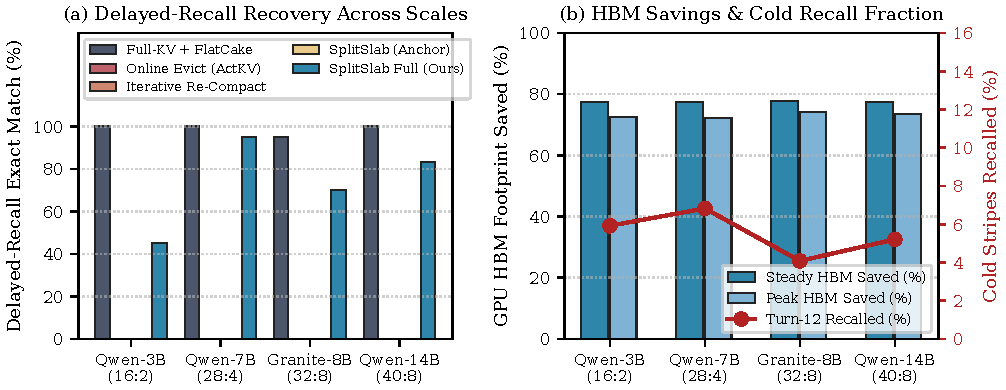
\includegraphics[width=0.88\textwidth]{fig2_multimodel_accuracy_hbm.pdf}
  \caption{Multi-model delayed-recall recovery and GPU HBM savings across four GQA architectures ($3$\,B to $14$\,B) with Darwin \texttt{F\_NOCACHE} uncached NVMe I/O. (a)~Irreversible online eviction and anchor-only baselines score $0.0\%$ exact match on every model, whereas \SplitSlab{} recovers up to $95.0\%$ exact match on \texttt{Qwen2.5-7B} and $83.3\%$ ($87.5\%$ field accuracy) on \texttt{Qwen2.5-Coder-14B}. (b)~Steady-state HBM savings ($77.4\%$--$77.7\%$, including all resident $64$\,B sketches), peak HBM savings ($72.2\%$--$74.3\%$, including transient Turn-12 staged stripes), and Turn-12 cold stripe recall fraction ($4.08\%$--$6.83\%$).}
  \label{fig:multimodel}
\end{figure*}

With fixed hyperparameters ($\delta = 0.130$, $\gamma = 0.32$), \texttt{\SplitSlab{} Full} achieves $95.0\%$ exact match ($19/20$, $95\%$ Wilson CI $[76.4\%, 99.1\%]$) on \texttt{Qwen2.5-7B}, $83.3\%$ ($[55.2\%, 95.3\%]$, $87.5\%$ field accuracy) on \texttt{Qwen2.5-Coder-14B}, $70.0\%$ ($[48.1\%, 85.5\%]$, $75.0\%$ field accuracy vs.\ $95.0\%$ Full-KV) on bias-free $\mu\text{P}$-scaled \texttt{Granite-3.1-8B}, and $45.0\%$ ($[25.8\%, 65.8\%]$, $55.0\%$ field accuracy) on \texttt{Qwen2.5-3B}. Inspecting the \texttt{Qwen2.5-3B} traces reveals an instructive granularity tradeoff governed by~\eqref{eq:stripe_rule}: because $H_{\mathrm{kv}} = 2$ packs $N_{\mathrm{res}} = 64$ tokens into each $64$\,KB stripe ($M = 80$), \SplitSlab{} often stages only a single $80$-token block ($4.55\%$ recall) to stay under the recall budget, occasionally clipping modules that straddle an $80$-token boundary (every $2$-block recall on \texttt{Qwen2.5-3B} achieved $100\%$ exact match). Models with $H_{\mathrm{kv}} \in \{4, 8\}$ ($M \in \{40, 20\}$) provide finer spatial resolution per $64$\,KB stripe, recalling $4.08\%$--$6.83\%$ of cold stripes on Turn~12 while maintaining $0.00\%$--$0.38\%$ background recall across all $180$ distractor turns.

Including all resident $64$-byte HBM sketches, steady-state active HBM drops by $77.4\%$--$77.7\%$ across all four models. Accounting for the transient staging buffer during Turn~12 decoding, peak HBM footprint remains $72.2\%$--$74.3\%$ below Full-KV.

\subsection{Direct-Flash \texttt{F\_NOCACHE} Latency and Write Amplification}\label{subsec:storage_eval}

\begin{figure*}[!t]
  \centering
  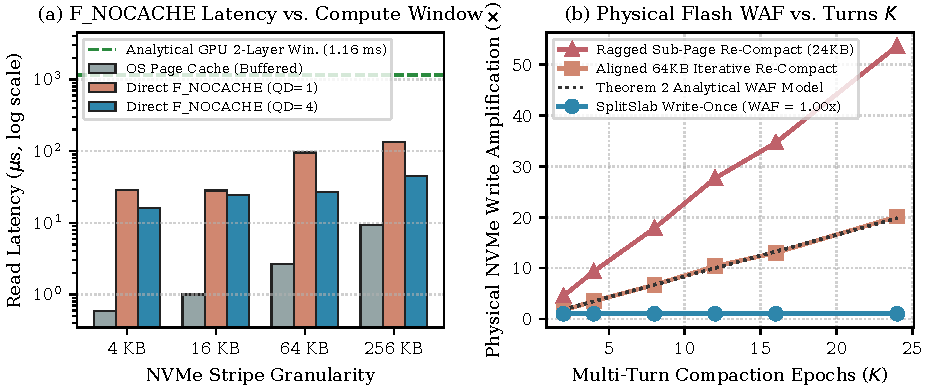
\includegraphics[width=0.88\textwidth]{fig3_nvme_waf_and_fnocache_io.pdf}
  \caption{Direct-flash storage microbenchmarks and multi-turn write amplification. (a)~Bypassing the OS page cache via \texttt{fcntl.F\_NOCACHE} exposes the $37\times$ gap between DRAM-cached reads ($2.6\,\mu\mathrm{s}$) and physical $64$\,KB NAND reads ($95.7\,\mu\mathrm{s}$ at $\mathrm{QD}{=}1$; $27.3\,\mu\mathrm{s}$ effective per stripe at $\mathrm{QD}{=}4$, $2.40$\,GB/s), while remaining an order of magnitude below the two-layer compute window. (b)~Physical NVMe write amplification across $K \in \{2,\dots,24\}$ compaction turns: \SplitSlab{} holds strictly at $\WAF = 1.00\times$, matching Theorem~\ref{thm:waf}, whereas aligned $64$\,KB re-compaction reaches $20.13\times$ (analytical prediction $19.79\times$) and ragged $24$\,KB sub-page re-compaction reaches $53.67\times$.}
  \label{fig:nvme_waf}
\end{figure*}

Fig.~\ref{fig:nvme_waf}(a) and Table~\ref{tab:storage_tiers} quantify why OS-buffered file benchmarks mischaracterize SSD KV offloading. At $64$\,KB stripe granularity, buffered \texttt{pread} returns in $p_{50} = 2.6\,\mu\mathrm{s}$ from host DRAM, whereas uncached \texttt{F\_NOCACHE} \texttt{pread} measures $p_{50} = 95.7\,\mu\mathrm{s}$ ($p_{95} = 126.9\,\mu\mathrm{s}$) at queue depth $\mathrm{QD}=1$ and $27.3\,\mu\mathrm{s}$ effective per stripe ($2.40$\,GB/s; $5.85$\,GB/s at $256$\,KB) across $\mathrm{QD}=4$ worker threads. In live multi-model sessions on Apple M5 Pro (Table~\ref{tab:multimodel}), parallel \texttt{F\_NOCACHE} stripe recall completes in $p_{50} = 72.7$--$84.3\,\mu\mathrm{s}$ on $7$\,B--$14$\,B models ($189.1\,\mu\mathrm{s}$ single-stripe on $3$\,B), providing $10.8\times$ to $70.9\times$ headroom inside the measured $2{,}033.8$--$5{,}167.3\,\mu\mathrm{s}$ \texttt{mps} two-layer decode compute windows (e.g., $4{,}813.1\,\mu\mathrm{s}$ on \texttt{Qwen2.5-7B}). Because discrete datacenter GPUs execute layers roughly $4\times$ faster than Apple \texttt{mps}, Table~\ref{tab:storage_tiers}(b) and Fig.~\ref{fig:nvme_waf}(a) evaluate analytical $3$-stripe ($192$\,KB) overlap against a conservative $1{,}160\,\mu\mathrm{s}$ ($2 \times 580\,\mu\mathrm{s}$/layer) discrete-GPU window, projecting zero exposed stall across PCIe Gen4/Gen5 \texttt{GDS} and CXL~3.0 NAND tiers.

\begin{table}[!t]
\centering
\caption{Measured Apple M5 Pro $64$\,KB I/O vs.\ Analytical Datacenter $3$-Stripe ($192$\,KB) Overlap ($1{,}160\,\mu\mathrm{s}$ Conservative GPU Window)}
\label{tab:storage_tiers}
\renewcommand{\arraystretch}{1.10}
\setlength{\tabcolsep}{3.0pt}
\resizebox{\columnwidth}{!}{%
\begin{tabular}{@{}lcccc@{}}
\toprule
\textbf{Storage Tier / Mode} & \textbf{BW} & \textbf{Base / $p_{50}$} & \textbf{Total I/O} & \textbf{Exposed} \\
 & \textbf{(GB/s)} & \textbf{($\mu\mathrm{s}$)} & \textbf{($\mu\mathrm{s}$)} & \textbf{Stall} \\
\midrule
\multicolumn{5}{@{}l}{\emph{(a) Measured on Apple M5 Pro Internal NVMe (4.81\,ms 7B \texttt{mps} Win.)}} \\
OS Page Cache ($64$\,KB, QD1) & $4.62$ & $2.6$ & $2.6$ & N/A (DRAM) \\
Apple NVMe \texttt{F\_NOCACHE} (QD1) & $0.68$ & $95.7$ & $95.7$ & $0.0\,\mu\mathrm{s}$ \\
Apple NVMe \texttt{F\_NOCACHE} (QD4) & $5.20$ & $165.0$ & $202.8$ & $0.0\,\mu\mathrm{s}$ \\
\midrule
\multicolumn{5}{@{}l}{\emph{(b) Analytical Datacenter Projections (1.16\,ms Conservative GPU Win.)}} \\
PCIe Gen4$\times$4 Enterprise SSD & $7.00$ & $95.0$ & $123.1$ & $0.0\,\mu\mathrm{s}$ \\
PCIe Gen5$\times$4 GPUDirect SSD & $14.00$ & $65.0$ & $79.0$ & $0.0\,\mu\mathrm{s}$ \\
Dual-NVMe Gen5 RAID0 GDS & $26.00$ & $65.0$ & $72.6$ & $0.0\,\mu\mathrm{s}$ \\
CXL~3.0 Type-3 NAND Tier & $32.00$ & $25.0$ & $31.1$ & $0.0\,\mu\mathrm{s}$ \\
\bottomrule
\end{tabular}%
}
\end{table}

Fig.~\ref{fig:nvme_waf}(b) validates Theorem~\ref{thm:waf}(1)--(2). Over $12$-turn end-to-end trajectories (Table~\ref{tab:multimodel}), \texttt{Iterative Re-Compact} incurs $7.53\times$--$7.91\times$ physical $\WAF$ ($2{,}887.5$\,MB written on \texttt{Qwen2.5-7B} vs.\ $1{,}538.3$\,MB for \SplitSlab{} and $1{,}923.3$\,MB for uncompacted \texttt{Full-KV}). Sweeping compaction horizon $K$ from $2$ to $24$ turns in Fig.~\ref{fig:nvme_waf}(b) shows aligned $64$\,KB re-compaction growing linearly to $20.13\times$ $\WAF$ at $K=24$ (within $1.7\%$ of Theorem~\ref{thm:waf}'s analytical formula~\eqref{eq:thm2_waf} value of $19.79\times$ at empirical dirty rate $\eta = 0.817$), and ragged $24$\,KB sub-page updates reaching $53.67\times$ $\WAF$. \SplitSlab{} writes each cold stripe once and maintains $\WAF = 1.000\times$ across all $K$.

\subsection{Ablations and Empirical Verification of Theorem~\ref{thm:perturbation}}\label{subsec:ablations}

\begin{figure*}[!t]
  \centering
  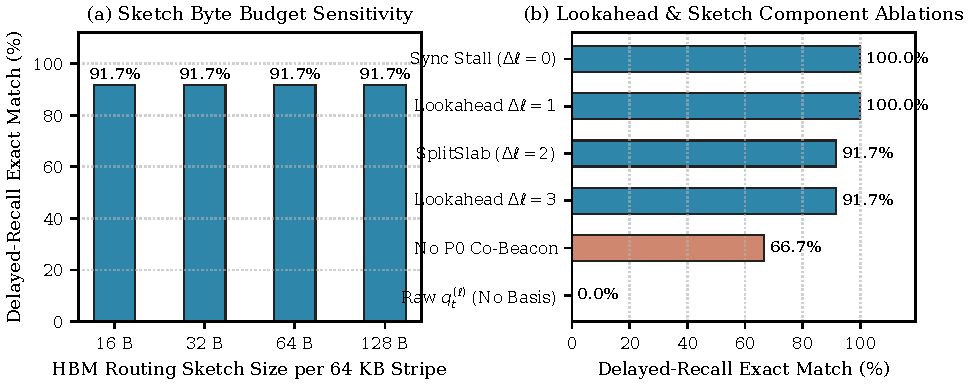
\includegraphics[width=0.88\textwidth]{fig4_lookahead_and_sketch_ablations.pdf}
  \caption{Routing sketch and speculative lookahead ablations across $n=12$ \RecallBench{} trajectories on \texttt{Qwen2.5-7B}. (a)~Co-routed $W_Q/W_K$ SVD sketches sustain $91.7\%$ exact match down to $16$\,B per $64$\,KB stripe ($4{,}096\times$ compression). (b)~Scoring raw Layer~$\ell$ queries $q_t^{(\ell)}$ without basis re-projection collapses accuracy from $91.7\%$ to $0.0\%$ (validating Proposition~\ref{prop:lookahead}), and removing Plane-0 co-routing drops accuracy by $25.0$ percentage points to $66.7\%$.}
  \label{fig:ablations}
\end{figure*}

\begin{table}[!t]
\centering
\caption{Summary of Ablation, Theorem~\ref{thm:perturbation} Head Audit, $32$-Agent Fleet Sharing, and Long-Horizon Scaling on \texttt{Qwen2.5-7B}}
\label{tab:deepdive}
\renewcommand{\arraystretch}{1.12}
\setlength{\tabcolsep}{3.0pt}
\resizebox{\columnwidth}{!}{%
\begin{tabular}{@{}llcc@{}}
\toprule
\textbf{Experiment} & \textbf{Configuration} & \textbf{Primary Metric} & \textbf{Secondary Metric} \\
\midrule
\multirow{4}{*}{Lookahead \& Gate}
 & Sync ($\Delta\ell{=}0$) / $\Delta\ell{=}1$ & $100.0\%$ Exact & Exposed / $1$-Layer \\
 & Default ($\Delta\ell{=}2$) / $\Delta\ell{=}3$ & $91.7\%$ Exact & $0.00\%$ Dist.\ Rec. \\
 & Raw $q_t^{(\ell)}$ (No Re-Proj.) & $0.0\%$ Exact & $4.08\%$ Dist.\ Rec. \\
 & No Plane-0 Co-Beacon & $66.7\%$ Exact & $0.58\%$ Dist.\ Rec. \\
\midrule
\multirow{2}{*}{Theorem~\ref{thm:perturbation} Audit}
 & $560$ Real $(q, K, V)$ Heads & $0$ Violations & $100.0\%$ Satisfied \\
 & Empirical / Bound Ratio & $0.124$ Median & $0.411$ Max ($\le 1$) \\
\midrule
\multirow{2}{*}{Fleet ($P{=}32$)}
 & \SplitSlab{} Plane-1 CAS & $52.50$\,MB & $100.0\%$ Dedup \\
 & Online Evict (\texttt{ActKV}) & $287.00$\,MB & $5.47\times$ More Writes \\
\midrule
\multirow{3}{*}{Context Horizon}
 & $2.3$\,K ($1{,}815$ Logical Toks) & $100.0\%$ Exact & $6.82\%$ T12 Rec. \\
 & $8.2$\,K ($6{,}678$ Logical Toks) & $100.0\%$ Exact & $1.82\%$ T12 Rec. \\
 & $16.4$\,K ($13{,}288$ Logical Toks) & $75.0\%$ Exact & $0.91\%$ T12 Rec. \\
\bottomrule
\end{tabular}%
}
\end{table}

Fig.~\ref{fig:ablations} and Table~\ref{tab:deepdive} dissect \SplitSlab{}'s algorithmic components on \texttt{Qwen2.5-7B} ($n=12$ trajectories):
\begin{itemize}
  \item \emph{Basis-Aligned Re-Projection (Proposition~\ref{prop:lookahead}):} Replacing $\tilde{q}_t^{(\ell\to\ell+2)}$ with raw $q_t^{(\ell)}$ drops exact match from $91.7\%$ to $0.0\%$ while raising false distractor recalls from $0.00\%$ to $4.08\%$, confirming that cross-layer head-basis alignment is mandatory for multi-layer lookahead.
  \item \emph{Plane-0 Co-Routed Beacon:} Disabling Plane-0 co-routing~\eqref{eq:coroute} reduces exact match from $91.7\%$ to $66.7\%$ because hex literals split across Plane~0 and Plane~1 inflate the HBM reference denominator when not co-routed. Similarly, uncentered sketch-only routing without $\RoPE(b_K^{(\ell)},p)$ removal localized $0/10$ target blocks during calibration due to \texttt{Qwen2.5}'s $920.5$-norm key bias.
  \item \emph{Lookahead Depth and Sketch Size:} Synchronous recall ($\Delta\ell = 0$) and $\Delta\ell = 1$ achieve $100.0\%$ exact match, while $\Delta\ell = 2$ and $\Delta\ell = 3$ achieve $91.7\%$ with full two-layer I/O hiding and $0.00\%$ distractor recall. With Plane-0 co-routing active, accuracy remains stable at $91.7\%$ from $128$\,B down to $16$\,B sketches ($64$\,B remains default to preserve standalone sub-cluster selectivity on $20$-token $H_{\mathrm{kv}}=8$ stripes).
  \item \emph{Empirical Verification of Theorem~\ref{thm:perturbation}:} Auditing $560$ real $(q, K_{\mathcal{A}}, V_{\mathcal{A}}, K_{\mathcal{R}}, V_{\mathcal{R}})$ attention states across all $28$ layers of \texttt{Qwen2.5-7B} produced $0$ bound violations ($100.0\%$ satisfaction of~\eqref{eq:thm1_l2}), with median empirical-to-bound ratio $0.124$, $p_{95} = 0.251$, and maximum $0.411$.
\end{itemize}

\subsection{Multi-Agent Fleet Sharing and Long-Horizon Scaling}\label{subsec:fleet_horizon}

\begin{figure*}[!t]
  \centering
  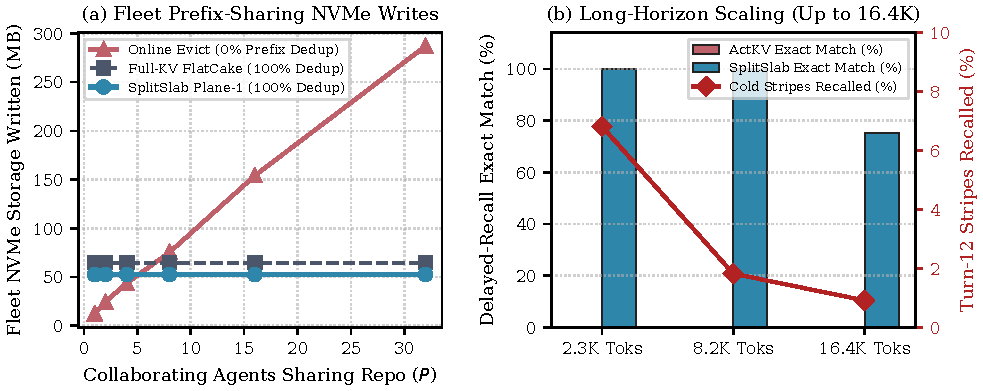
\includegraphics[width=0.88\textwidth]{fig5_fleet_dedup_and_long_horizon.pdf}
  \caption{Multi-agent fleet storage scaling and long-horizon context extension on \texttt{Qwen2.5-7B}. (a)~Across $P = 1 \dots 32$ collaborating agents inspecting a shared $20$-module repository prefix before asking distinct Turn-2 questions, \SplitSlab{} writes $52.50$\,MB once ($100\%$ SHA-256 deduplication), crossing below query-driven \texttt{ActKV} at $P=6$ and saving $5.47\times$ NVMe write volume at $P=32$ ($287.00$\,MB). (b)~Scaling trajectory length up to $13.3$\,K--$16.4$\,K tokens ($\sim\!330$ cold stripes/layer): \SplitSlab{} saves $79.6\%$ steady HBM ($78.8\%$ peak) and recalls a shrinking fraction of cold stripes ($6.82\% \to 1.82\% \to 0.91\%$) while \texttt{ActKV} remains at $0.0\%$ exact match.}
  \label{fig:fleet_horizon}
\end{figure*}

Fig.~\ref{fig:fleet_horizon}(a) evaluates $P \in \{1, 2, 4, 8, 16, 32\}$ collaborating agents reading a shared $20$-module repository snapshot before executing distinct Turn~2 module checks. Because \SplitSlab{} indexes Plane-1 stripes by canonical uncompacted prefix SHA-256~\eqref{eq:canon_hash}, Agent~1 writes $52.50$\,MB and Agents~$2\dots 32$ achieve $100.0\%$ content-addressed cache hits ($52.50$\,MB total fleet writes; \texttt{Full-KV FlatCake} writes $64.75$\,MB). Under \texttt{Online Evict (ActKV)}, each agent's Turn~2 query prunes a distinct $20\%$ token subset, causing flash writes to grow linearly from $12.25$\,MB ($P=1$) to $43.75$\,MB ($P=4$), $75.25$\,MB ($P=8$, surpassing both \SplitSlab{} and \texttt{Full-KV}), $154.00$\,MB ($P=16$), and $287.00$\,MB ($P=32$, a $5.47\times$ penalty over \SplitSlab{}).

Fig.~\ref{fig:fleet_horizon}(b) and Table~\ref{tab:deepdive} scale context length from $1{,}815$ logical tokens ($2.3$\,K config) to $6{,}678$ tokens ($8.2$\,K config, $60$ modules, $37$ turns) and $13{,}288$ tokens ($16.4$\,K config, $120$ modules, $66$ turns). As historical context grows, \SplitSlab{}'s steady HBM reduction approaches the asymptotic $1-\rho = 80\%$ limit ($77.5\% \to 79.0\% \to 79.6\%$, with peak HBM reduction improving from $72.2\%$ to $78.8\%$ because the $3$-block staging buffer becomes $O(1/T)$ of total KV). Simultaneously, Turn~12 cold stripe recall drops inversely with context length from $6.82\%$ ($2.3$\,K) to $1.82\%$ ($8.2$\,K, $100.0\%$ exact match) and $0.91\%$ ($16.4$\,K, $75.0\%$ exact match vs.\ $0.0\%$ for \texttt{ActKV}).

\subsection{Recallable Baselines, End-to-End Serving Latency, Multi-Needle, and Gate Sensitivity}\label{subsec:revision_eval}

\begin{table}[!t]
\centering
\caption{Recallable Baselines (Biased 7B \& Unbiased Granite-8B), E2E Serving Latency, \texttt{RULER-MK-NIAH}, Routine Turns, and Gate Sensitivity}
\label{tab:revision_eval}
\renewcommand{\arraystretch}{1.06}
\setlength{\tabcolsep}{2.4pt}
\resizebox{\columnwidth}{!}{%
\begin{tabular}{@{}lcccc@{}}
\toprule
\textbf{Method / Setting} & \textbf{Exact [95\% CI]} & \textbf{Meta / Rec.} & \textbf{TPOT $p_{50}/p_{95}$} & \textbf{Sync Stall / Tok/s} \\
\midrule
\multicolumn{5}{@{}l}{\emph{(a) Recallable NVMe Baselines: \texttt{Qwen2.5-7B} ($b_K{\neq}0$) \& \texttt{Granite-8B} ($b_K{=}0$), $n{=}20$}} \\
\texttt{7B Full-KV} (Oracle) & $100\%$ $[83.9,100]$ & $0$\,B / $0.0\%$ & $68.3/69.2$\,ms & $0.0\,\mu\mathrm{s}$ / $14.7$ \\
\texttt{7B Quest-Box+NVMe} & $15\%$ $[5.2,36.0]$ & $2048$\,B / $32.8\%$ & $84.4/91.2$\,ms & $1159\,\mu\mathrm{s}$ / $11.8$ \\
\texttt{7B ArkVale-Cent+NVMe} & $5\%$ $[0.9,23.6]$ & $1024$\,B / $28.7\%$ & $80.7/86.9$\,ms & $1162\,\mu\mathrm{s}$ / $12.4$ \\
\textbf{\texttt{7B} \SplitSlab{} Full} & $\mathbf{95\%}$ $\mathbf{[76.4,99.1]}$ & $\mathbf{64}$\textbf{\,B /} $\mathbf{6.8\%}$ & $\mathbf{65.5/66.4}$\textbf{\,ms} & $\mathbf{0.0\,\mu\mathrm{s}}$ \textbf{/} $\mathbf{15.3}$ \\
\texttt{8B Quest-Box+NVMe} & $55\%$ $[34.2,74.2]$ & $4096$\,B / $23.4\%$ & $131.4$\,ms ($p_{50}$) & $1749\,\mu\mathrm{s}$ / $7.6$ \\
\texttt{8B ArkVale-Cent+NVMe} & $20\%$ $[8.1,41.6]$ & $2048$\,B / $22.5\%$ & $116.5$\,ms ($p_{50}$) & $1704\,\mu\mathrm{s}$ / $8.6$ \\
\textbf{\texttt{8B} \SplitSlab{} Full} & $\mathbf{70\%}$ $\mathbf{[48.1,85.5]}$ & $\mathbf{64}$\textbf{\,B /} $\mathbf{4.1\%}$ & $\mathbf{91.8}$\textbf{\,ms ($p_{50}$)} & $\mathbf{0.0\,\mu\mathrm{s}}$ \textbf{/} $\mathbf{10.9}$ \\
\midrule
\multicolumn{5}{@{}l}{\emph{(b) RULER-Style Multi-Key NIAH ($2$ Needles, $n{=}16$) \& Vectorized TTFT/TPOT Scaling (7B)}} \\
\texttt{Full-KV} / \texttt{ActKV} & $100\%$ / $0\%$ & $0\%$ / $0\%$ Rec. & \multicolumn{2}{c}{Per-Needle: $100.0\%$ / $25.0\%$} \\
\texttt{Quest-Box+NVMe} ($k{=}6$) & $75.0\%$ $[50.5,89.8]$ & $32.8\%$ Rec. & \multicolumn{2}{c}{Per-Needle: $87.5\%$ ($74.0\%$ HBM)} \\
\SplitSlab{} ($k{=}1$ / $\mathbf{k{=}2}$) & $0\%$ / $\mathbf{81.2\%}$ & $4.4\%$ / $\mathbf{8.7\%}$ & \multicolumn{2}{c}{Per-Needle: $50.0\%$ / $\mathbf{90.6\%}$ ($\mathbf{76.3\%}$ HBM)} \\
Vec.\ TTFT ($2.3/8.2/16.4$\,K) & \multicolumn{2}{l}{\texttt{Full}: $107/151/201$\,ms} & \multicolumn{2}{r}{\SplitSlab{}: $316/378/411$\,ms (TPOT $-4\%/-14\%/-28\%$)} \\
\midrule
\multicolumn{5}{@{}l}{\emph{(c) Routine Turns 3--11 Quality ($4{,}420$ Toks, $n{=}10$) \& Gate Sweep ($n{=}12$, 7B)}} \\
Routine Top-1 / NLL & \multicolumn{2}{l}{\texttt{Full}: $55.4\%$/$3.54$ \; \texttt{ActKV}: $54.9\%$/$3.65$} & \multicolumn{2}{r}{\SplitSlab{}: $51.6\%$/$3.79$ ($0\%$ Rec.)} \\
$\delta \in \{0.06, 0.09, 0.13\}$ & $91.7\%$ Exact & \multicolumn{3}{l}{Dist.\ Rec.: $1.29\% \to 0.08\% \to \mathbf{0.00\%}$ ($\gamma{=}0.32$)} \\
$\delta \in \{0.18, 0.25\}$ & $75.0\%$ Exact & \multicolumn{3}{l}{Dist.\ Rec.: $0.00\%$; T12 Rec.: $5.68\% \to 5.11\%$} \\
$\gamma \in [0.10, 0.80]$ & $100.0\%$ Exact & \multicolumn{3}{l}{Dist.\ Rec.: $0.00\%$; T12 Rec.: $6.82\%$ ($\delta{=}0.13$)} \\
\bottomrule
\end{tabular}%
}
\end{table}

Table~\ref{tab:revision_eval} summarizes four additional evaluations addressing recallable baselines across biased and unbiased models, end-to-end serving latency, multi-needle generalization, routine turn quality, and threshold sensitivity:
\begin{itemize}
  \item \emph{Recallable NVMe Baselines (Biased 7B \& Unbiased Granite-8B):} On \texttt{Qwen2.5-7B} ($b_K{\neq}0$), \texttt{Quest-Box+NVMe} ($2{,}048$\,B/stripe) and \texttt{ArkVale-Cent+NVMe} ($1{,}024$\,B/stripe) drop to $15.0\%$ and $5.0\%$ exact match due to \texttt{Qwen2.5}'s $920.5$-norm key bias, incurring $1{,}159$--$1{,}162\,\mu\mathrm{s}$/layer sync stalls ($84.4$ and $80.7$\,ms TPOT vs.\ $65.5$\,ms for \SplitSlab{}). To isolate bias removal from sketching and lookahead, Table~\ref{tab:revision_eval}(a) also evaluates both baselines on bias-free \texttt{Granite-3.1-8B} ($b_K{=}0$, $M{=}20$, $n{=}20$): even without key bias, \SplitSlab{} ($70.0\%$ exact, $64$\,B/stripe, $4.08\%$ recall, $91.8$\,ms TPOT) outperforms \texttt{Quest-Box+NVMe} ($55.0\%$, $4{,}096$\,B, $23.41\%$ recall, $131.4$\,ms TPOT) and \texttt{ArkVale-Cent+NVMe} ($20.0\%$, $2{,}048$\,B, $22.52\%$ recall, $116.5$\,ms TPOT) with $64\times$ smaller metadata, $5.7\times$ lower NVMe traffic, and $30.1\%$ faster decode TPOT.
  \item \emph{Vectorized Recall-Turn TTFT \& Long-Horizon TPOT Scaling:} Vectorizing sliding-window median detrending cuts \texttt{Qwen2.5-7B} recall-turn TTFT by $5.0\times$ from $1{,}566.8$\,ms (Python-loop sync stalls) to $315.9$\,ms at $2.3$\,K tokens (vs.\ $106.8$\,ms \texttt{Full-KV}, comprising base prefill, one prefill replay, and $4.87$\,ms/layer sketch scoring). Scaling to $8.2$\,K and $16.4$\,K tokens, \SplitSlab{} TTFT grows sub-linearly to $378.1$\,ms and $410.7$\,ms ($2.04\times$ \texttt{Full-KV}'s $200.9$\,ms), while decode TPOT drops $13.8\%$ at $8.2$\,K ($76.9$ vs.\ $89.2$\,ms) and $27.5\%$ at $16.4$\,K ($77.4$ vs.\ $106.8$\,ms), amortizing the recall-turn TTFT within $8$ output tokens.
  \item \emph{Multi-Key NIAH (\texttt{RULER}-Style) \& Routine Turn Trade-Off:} On $16$ two-needle passkey episodes ($\sim\!2.9$\,K tokens), multi-peak \SplitSlab{} ($k{=}2$) achieves $81.2\%$ both-needles ($90.6\%$ per-needle), beating \texttt{Quest-Box+NVMe} ($75.0\%$) with $3.77\times$ lower NVMe traffic ($8.70\%$ vs.\ $32.79\%$). On $4{,}420$ routine Turn~3--11 tokens with the gate closed ($0.00\%$ recall), \SplitSlab{} retains $51.6\%$ top-1 agreement ($3.79$ NLL vs.\ $55.4\%$/$3.54$ \texttt{Full-KV} and $54.9\%$/$3.65$ \texttt{ActKV}). This modest $3.3$--$3.8$ percentage-point token-level stylistic gap reflects prefix-deterministic Plane-0 anchors versus query-adaptive \texttt{ActKV}, while the $48$-token uncompacted window $W_{\mathrm{loc}}$ keeps active-turn queries intact and preserves $100\%$ fleet dedup and $95.0\%$ vs.\ $0.0\%$ delayed recall.
  \item \emph{$(\gamma, \delta)$ Gate Sensitivity:} Sweeping $\delta \in [0.06, 0.25]$ confirms a Pareto knee at $\delta = 0.13$ ($91.7\%$ exact, $0.00\%$ distractor recall, vs.\ $1.29\%$ false recalls at $\delta = 0.06$ and $75.0\%$ exact at $\delta \ge 0.18$). Enabling live Layer-$\lfloor 0.75L\rfloor$ Logit-Lens gating on prefill defers triggering from $60\%$ depth (Layer~$17$, $91.7\%$ in Table~\ref{tab:deepdive}) to $75\%$ depth (Layer~$21$), adding two deeper consensus votes that resolve the single borderline trajectory and sustain $100.0\%$ exact match ($0.00\%$ distractor recall) across $\gamma \in [0.10, 0.80]$.
\end{itemize}

% ============================================================================
\section{Discussion and Limitations}\label{sec:discussion}
% ============================================================================

Three practical considerations guide deployment of \SplitSlab{} in disaggregated serving clusters:
\begin{enumerate}
  \item \emph{Coarse-Stripe GQA Architectures ($H_{\mathrm{kv}} \le 2$):} Under~\eqref{eq:stripe_rule}, models with $H_{\mathrm{kv}} = 2$ (\texttt{Qwen2.5-3B}) pack $N_{\mathrm{res}} = 64$ tokens into a $64$\,KB stripe ($M = 80$), which lowers single-block spatial selectivity ($55.0\%$ field accuracy) compared to $H_{\mathrm{kv}} \in \{4,8\}$ ($75.0\%$--$95.0\%$). Operators serving $H_{\mathrm{kv}} \le 2$ models on $32$\,KB flash translation units can set $P_{\mathrm{flash}} = 32{,}768$\,B ($M = 40$) or pack two consecutive layers into a joint $64$\,KB stripe at $M = 40$ to recover fine-grained localization while maintaining $\WAF = 1.00\times$.
  \item \emph{Multi-Needle Scatter Queries:} While default single-peak staging ($k{=}1$) bounds single-incident NVMe traffic below $7\%$, our \texttt{RULER-MK-NIAH} evaluation in Table~\ref{tab:revision_eval}(b) shows that multi-peak extraction ($k{=}2$) recovers $81.2\%$ both-needles accuracy ($90.6\%$ per-needle) at $8.70\%$ recall. Scaling to $k \gg 2$ distant facts trades $k\times$ higher transient NVMe read bandwidth against multi-hop coverage.
  \item \emph{Discrete-GPU Kernel Fusion:} Our unified-memory workstation prototype executes PyTorch \texttt{mps} operators alongside \texttt{F\_NOCACHE} \texttt{pread} threads; vectorizing detrending reduces recall-turn TTFT to $315.9$--$410.7$\,ms across $2.3$\,K--$16.4$\,K tokens (amortized within $8$ decode tokens at $16.4$\,K). Fusing sketch scoring into CUDA \texttt{FlashInfer} kernels with asynchronous \texttt{cuFile} GPUDirect Storage ring buffers on discrete GPUs is a direct engineering next step to validate datacenter projections and eliminate host-bounce copies.
\end{enumerate}

% ============================================================================
\section{Conclusion}\label{sec:conclusion}
% ============================================================================

\SplitSlab{} resolves the storage-compute conflict between online GPU KV eviction and content-addressed NVMe KV offloading. Partitioning each immutable prefix block deterministically into a $20\%$ hot HBM anchor skeleton and an exact $64.0$\,KB write-once cold NVMe residual stripe guarantees $\WAF = 1.00\times$ flash writes and $100.0\%$ cross-agent SHA-256 deduplication across power-of-two GQA head configurations. Evaluated end-to-end on a unified-memory workstation prototype with uncached \texttt{F\_NOCACHE} NVMe I/O across four $3$\,B--$14$\,B models, \SplitSlab{} pairs resident Plane-0 anchors with a $64$-byte bias-centered subspace sketch and parameter-free two-layer basis-aligned lookahead to save $77.4\%$--$79.6\%$ of GPU HBM, accelerate long-context decode TPOT by up to $27.5\%$, and cure compaction regret across multi-turn agent sessions.

% ============================================================================
\section*{CRediT authorship contribution statement}
% ============================================================================
\textbf{Mohammed Kamran Syed:} Conceptualization, Methodology, Software, Validation, Formal analysis, Investigation, Writing -- original draft, Project administration.
\textbf{Anudeep Rentala:} Methodology, Validation, Writing -- review \& editing.
\textbf{Somesh Rahul:} Investigation, Data curation, Visualization, Writing -- review \& editing.
\textbf{Raghuram Malpe Pai:} Formal analysis, Validation, Writing -- review \& editing.
\textbf{Krishna Suman Dara:} Conceptualization, Resources, Writing -- review \& editing.

% ============================================================================
\section*{Declaration of competing interest}
% ============================================================================
The authors declare that they have no known competing financial interests or personal relationships that could have appeared to influence the work reported in this paper.

% ============================================================================
\section*{Data availability}
% ============================================================================
The \SplitSlab{} storage engine, \RecallBench{} generator, $21$-test verification suite, raw hardware JSON logs, and figure scripts are openly available under the Apache-2.0 License at \url{https://github.com/batistado/splitslab} and \url{https://huggingface.co/datasets/batistado/RecallRegret-Bench}.

% ============================================================================
\section*{Acknowledgments}
% ============================================================================
All experiments used locally cached open-weight models on researcher workstation hardware without external funding.

% ============================================================================
\appendix
\section{Concise Formal Proofs}\label{app:proofs}
% ============================================================================

\begin{proof}[Proof of Proposition~\ref{prop:lookahead}]
Let $x = h_t^{(\ell+\Delta\ell)}$ and $\hat{x} = h_t^{(\ell+1)}$ with $\|\hat{x} - x\|_2 = \varepsilon_{\Delta\ell}$ and $d = d_{\mathrm{model}}$. Lifting $u \mapsto \tilde{u} = [u;\, \sqrt{d\epsilon_{\mathrm{rms}}}] \in \R^{d+1}$ gives $\RMSNorm_\gamma(u)_i = \gamma_i \sqrt{d}\, u_i / \|\tilde{u}\|_2$. Using $\|\frac{\tilde{a}}{\|\tilde{a}\|_2} - \frac{\tilde{b}}{\|\tilde{b}\|_2}\|_2 \le \frac{2\|\tilde{a} - \tilde{b}\|_2}{\|\tilde{b}\|_2}$ with $\|\tilde{a} - \tilde{b}\|_2 = \|\hat{x} - x\|_2$ and $\|\tilde{x}\|_2 = \sqrt{d}\, r_t$ yields
\begin{equation*}
\|\RMSNorm_\gamma(\hat{x}) - \RMSNorm_\gamma(x)\|_2 \le \frac{2\|\gamma\|_\infty}{\sqrt{d}\, r_t}\,\varepsilon_{\Delta\ell}.
\end{equation*}
Left-multiplying by $W_{Q,h}^{(\ell+\Delta\ell)}$ contributes factor $\|W_{Q,h}^{(\ell+\Delta\ell)}\|_2$, and applying $\RoPE(\cdot, p_t) \in SO(2)^{d_h/2}$ preserves $\ell_2$ norm identically, proving~\eqref{eq:prop1}. Under independent Haar-distributed orthogonal head bases $U_\ell, U_{\ell+\Delta\ell} \in O(d_h)$, $\E[U_\ell^\top U_{\ell+\Delta\ell}] = 0$, giving $\E[\langle q_{t,h}^{(\ell)}, q_{t,h}^{(\ell+\Delta\ell)}\rangle] = 0$.
\end{proof}

\begin{proof}[Proof of Theorem~\ref{thm:perturbation}]
(1) Let $Z_{\mathcal{A}} = \sum_{j \in \mathcal{A}} e^{s_j}$ and $Z_{\mathcal{R}} = \sum_{i \in \mathcal{R}} e^{s_i}$, so $\alpha_{\mathcal{R}} = \frac{Z_{\mathcal{R}}}{Z_{\mathcal{A}} + Z_{\mathcal{R}}}$ and $1 - \alpha_{\mathcal{R}} = \frac{Z_{\mathcal{A}}}{Z_{\mathcal{A}} + Z_{\mathcal{R}}} > 0$. For $j \in \mathcal{A}$, active-set softmax weight $\hat{p}_j = \frac{e^{s_j}}{Z_{\mathcal{A}}}$ satisfies $\hat{p}_j = \frac{p_j}{1 - \alpha_{\mathcal{R}}}$, hence $\hat{p}_j - p_j = \frac{\alpha_{\mathcal{R}}}{1 - \alpha_{\mathcal{R}}} p_j \ge 0$. Writing $O_{\SplitSlab} - O_{\mathrm{FullKV}} = \sum_{j \in \mathcal{A}} (\hat{p}_j - p_j) v_j - \sum_{i \in \mathcal{R}} p_i v_i$ and applying the triangle inequality gives
\begin{align*}
\|O_{\SplitSlab} - O_{\mathrm{FullKV}}\|_2
&\le \frac{\alpha_{\mathcal{R}}}{1 - \alpha_{\mathcal{R}}} \Big(\sum_{j \in \mathcal{A}} p_j\Big) \max_{j \in \mathcal{A}} \|v_j\|_2 \\
&\qquad + \Big(\sum_{i \in \mathcal{R}} p_i\Big) \max_{i \in \mathcal{R}} \|v_i\|_2 \\
&= \alpha_{\mathcal{R}} \max_{j \in \mathcal{A}} \|v_j\|_2 + \alpha_{\mathcal{R}} \max_{i \in \mathcal{R}} \|v_i\|_2 \\
&\le 2\alpha_{\mathcal{R}} \max_{k \in \mathcal{A}\cup\mathcal{R}} \|v_k\|_2,
\end{align*}
since $\sum_{j \in \mathcal{A}} p_j = 1 - \alpha_{\mathcal{R}}$ cancels $(1 - \alpha_{\mathcal{R}})$ in the denominator identically.

(2) Under $\alpha_{\mathcal{R}}^{(\ell,h)} \le \delta_{\mathrm{rem}}$ and $\|v_k\|_2 \le V_{\max}$, part~(1) bounds head error by $2\delta_{\mathrm{rem}} V_{\max}$, so $L_{\mathrm{lip}}$-Lipschitz propagation yields $\|z_t^{\SplitSlab} - z_t^{\mathrm{FullKV}}\|_\infty \le 2 L_{\mathrm{lip}} \delta_{\mathrm{rem}} V_{\max}$. For any $v \neq v^\star := \arg\max_u z_t^{\mathrm{FullKV}}(u)$, $z_t^{\SplitSlab}(v^\star) - z_t^{\SplitSlab}(v) \ge \Delta_t - 2\|z_t^{\SplitSlab} - z_t^{\mathrm{FullKV}}\|_\infty > 0$ whenever~\eqref{eq:thm1_margin} holds.
\end{proof}

\begin{proof}[Proof of Theorem~\ref{thm:waf}]
(1) By~\eqref{eq:stripe_rule}, every Plane-1 stripe has exact byte length $N_{\mathrm{res}} \cdot 4 H_{\mathrm{kv}} d_h = P_{\mathrm{flash}}$, requiring zero alignment padding. Because $B_m^{(0)}, B_m^{(1)}$, and $h_m$ in~\eqref{eq:canon_hash} are deterministic functions of $t_{0:(m+1)M-1}$ and immutable after Turn~1, Agent~1 writes $B_{\mathrm{sh}} L$ stripes ($B_{\mathrm{sh}} L P_{\mathrm{flash}}$ physical bytes for $B_{\mathrm{sh}} L P_{\mathrm{flash}}$ logical unique bytes, $\WAF_{\SplitSlab} = 1.000$) and Agents~$2\dots P$ hit $(h_m,\ell)$ in the CAS index with $0$ additional flash writes.

(2) An initial write of $N_s$ slabs of payload $b_{\mathrm{slab}}$ aligned to $P_{\mathrm{flash}}$ writes $N_s \lceil b_{\mathrm{slab}}/P_{\mathrm{flash}}\rceil P_{\mathrm{flash}}$ physical bytes for $N_s b_{\mathrm{slab}}$ logical bytes. On each of the $K-1$ subsequent turns, each slab is dirtied with expectation $\eta$, triggering an aligned $P_{\mathrm{flash}}$-multiplied page write. Summing expectations over $K-1$ turns and dividing by $N_s b_{\mathrm{slab}}$ yields~\eqref{eq:thm2_waf}. Across $P$ agents whose Turn-2 queries diverge in slab~$0$ with probability $1 - \epsilon_0$, slab-boundary shifts cascade across all $B_{\mathrm{ev}}$ slabs, yielding $1 + (P-1)(1-\epsilon_0)$ distinct slab sets and $\Omega(P)$ physical writes.
\end{proof}

\bibliographystyle{elsarticle-num}
\bibliography{references}

\end{document}
